\chapter{Obstructed atomic limits in two dimensions}
\label{ch:oals}
In the Chapter~\ref{ch:tci}, we have shown that crystal symmetries may give rise to a wide range of novel topological states of quantum matter dubbed topological crystalline insulators. However, an even more striking consequence of the spatial symmetries is that several adiabatically disconnected atomic limits -- electronic phases in which all orbitals are fully localized -- can exist. While multiple atomic limits can be discerned, a topological distinction between these bulk phases is only relative and a choice which one has to be labeled as a trivial is arbitrary~\cite{PhysRevLett.114.177204}. These systems can be understood using an intuitive picture of atomic-like Wannier functions~\cite{PhysRev.52.191, MarziariWF2012}. The Wannier functions (WFs), which we present in more details in Appendix~\ref{ch:app_wannier}, are constructed from the isolated group of occupied Bloch bands of an insulator. In atomic limits, WFs are exponentially localized and verify the symmetries of the system. Most often, the center of electronic WFs coincide with atomic positions in a lattice, which we call a \emph{trivial atomic limit}. However, a hybridization between atomic orbitals may result in WFs localized far from the atomic sites. The latter situation is referred to as an \emph{obstructed atomic limit} (OAL)~\cite{Bradlyn17}, where the localized orbitals reside at the (maximal) Wyckoff positions\footnote{A Wyckoff position $w$ is a generic location in a unit cell such that it has its own site-symmetry (or point-symmetry) group $\mathcal{G}_w$, which is a subgroup of the crystal space group $\mathcal{G}$: $\mathcal{G}_w = \lbrace g = \lbrace p_g | \mathbf{r}_g \rbrace \in \mathcal{G} |  p_g \mathbf{r}_w + \mathbf{r}_g = \mathbf{r}_w \rbrace$, where $\mathbf{r}_w$ is the position of the Wyckoff position (we use here the Wigner-Seitz notation). In particular, a maximal Wyckoff position is defined as a point where the site-symmetry group is a maximal subgroup of $\mathcal{G}$.}. 

Conversely, topological phases characterized by a non-vanishing strong topological index such as Chern number cannot be expressed in terms of localized WFs as they exhibit extended edge modes in an open geometry associated with a bulk topology. In other words, a non-zero Chern number imposes a topological obstruction for deforming the ground state into a product state and, as a consequence, to the construction of exponentially localized WFs~\cite{Thouless_1984, PhysRevB.74.235111}. The opposite statement -- a vanishing topological index implies that a system can be described in terms of WFs -- was proven as well~\cite{PhysRevLett.98.046402}. In the case of $\mathbb{Z}_2$ topological insulators, a topological obstruction still applies if a gauge is chosen such that the time-reversal symmetry is preserved and the Wannier states come in time-reversal symmetric pairs~\cite{PhysRevB.83.035108}. It is important to note that obstructions to the Wannier representation does not always guarantee a stable topology, giving rise to the notion of \emph{fragile} topology~\cite{PhysRevLett.121.126402,BarryFragile,Bouhon18Fragile,KoreanTBG,wieder2018axion,MaiaFragile1,MaiaFragile2,MaiaFragile3}. Three types of (spatial) symmetry-protected phases: (i) stable topological, (ii) fragile topological, and (iii) obstructed limits are compared in Table~\ref{tab:topo-triv}.

\begin{table}[htbp]
\centering
\begin{tabularx}{\linewidth}{|  Y| Y  |Y | Y | Y | }
\hline 
System & Trivial atomic limit & Obstructed atomic limit & Fragile topological & Stable topological \\ 
\hline 
Wannier representable & yes & yes & no & no \\ 
\hline 
Trivialization by extra degrees of freedom & - & adding unoccupied bands & adding occupied bands & -  \\ 
\hline
Example & atomic insulator & see Sec.~\ref{sec:materials} & twisted bilayer graphene~\cite{KoreanTBG, PhysRevLett.123.036401, PhysRevB.99.195455} & Chern insulators, $Z_2$ TIs \\
\hline
\end{tabularx}
\caption[Classification of the band structures corresponding to the (spatial) symmetry-protected phases]{Classification of the band structures corresponding to the (spatial) symmetry-protected phases. All the band structures fall into two categories: \emph{topological} bands, which do not admit representation in terms of Wannier functions, and \emph{atomic} bands, for which the Wannier functions are exponentially localized. Within these two groups, a further distinction is possible. Fragile topological systems can be trivialized into a product state by adding occupied states, \ie, electrons, resulting in the change of the total filling. Adding empty bands to a system realizing an obstructed atomic limit, in which the WFs are located far from the positions of atoms, leads to its trivialization.}
\label{tab:topo-triv}
\end{table} 

OALs can support point-like boundary states in an open geometry, since the physical boundary of the system may result in 'cutting through' the Wannier centers. At fixed bulk filling, these \emph{dangling} Wannier charge centers become fractionally filled, which allows to define fractional charges~\cite{miertOrtixFractionalCharge17,miertcorners,EzawaWannier19,benalcazar2018quantization,GDY22019,GDY12019}. Hence, OALs can be perceived as examples of the so-called higher-order topology, which generalizes the bulk-boundary correspondence: a $d$-dimensional system with a non-trivial bulk topology exhibits boundary modes in a $(d-D)$ dimensions, with a co-dimension $D > 1$~\cite{BABHughesBenalcazar17,PhysRevLett.119.246401,HOTI12018,Benalcazar17, Song17,Khalaf18,Geier18,BenMoTe2}. The relation between 2D Wannier centers and corner charge was developed in Refs.~\cite{Song17,miertcorners,benalcazar2018quantization}. In particular, Ref.~\cite{benalcazar2018quantization} uses the algebraic structure of the classifications of $C_n$-symmetric insulators in class AI to build topological indices for corner charge. It has also been recently found that fragile topological phases can also host corner charges~\cite{benalcazar2018quantization,wieder2018axion} and that 2D second-order topological insulators also exhibit fractional charges at the core of defects with curvature singularities in both spinless and spinful insulators~\cite{benalcazar2018quantization,PhysRevX.9.031003,li2019fractional}.

In the absence of internal symmetries, though, $\mathrm{0D}$ states can be pushed out of the bulk gap and hybridized with bulk states by symmetry-preserving potential terms, which destroys their exponential localization. It is in contrast to the first-order phases in which 1D protected edge states demonstrate a spectral flow connecting conduction and valence bands. To define topology in a meaningful way, we employ a notion of a \emph{filling anomaly}~\cite{benalcazar2018quantization}: a topological property of the occupied bands of TCIs that counts the mismatch between the number of electrons needed to simultaneously satisfy charge neutrality and preserve the crystal symmetry. If the system with periodic boundary conditions is at the filling corresponding to an insulating band gap, then it has to be metallic with open boundary conditions when all relevant symmetries are respected. Importantly, this notion does not require a spectral symmetry, which is often used to pin boundary modes in the middle of a band gap. 

In general, a set of occupied bands (without strong or fragile topology) can be decomposed into subsets of bands stemming from localized orbitals at different Wyckoff positions. Such a set of bands is called a \emph{band representation}~\cite{Bradlyn17}. The minimal subblocks that cannot be further decomposed are \emph{elementary band representations} (EBRs), which are a connected set of subbands induced from placing a certain orbital at a given Wyckoff position~\cite{Slager12,Slager17,Bradlyn17,Cano17,Cano17-2,BarryFragile,ZakEBR1,ZakEBR2}. For the band representations, the irreducible representations (irreps) of the little group\footnote{A set of symmetry operations $g \in \mathcal{G}$ that leaves a momentum $\mathbf{k}$ invariant up to a reciprocal lattice vector $G$ is called little group $G_{\mathbf{k}}$ of $\mathbf{k}$: $G_{\mathbf{k}} = \lbrace g = \lbrace p_g | \mathbf{r}_g \rbrace \in \mathcal{G} | p_g \mathbf{k} \approx \mathbf{k} \rbrace$.} at high symmetry points (HSPs) in the BZ are completely determined by the irreps of the site-symmetry group under which the Wannier functions transform. Ref.~\cite{Bradlyn17} introduced EBRs as a means to discern bands that stem entirely from atomic limits from those with strong or fragile topology. Following the approach in Ref.~\cite{benalcazar2018quantization}, we use the additive structure of atomic limits that they provide to establish the correspondence between bulk invariants and corner charges sourced by OAL Wannier charge centers.

In this Chapter, we provide a classification of OALs and formulas for corner charges for all layer groups\footnote{Layer groups are extensions of two-dimensional possible plane symmetry groups called the wallpaper groups with an additional reflection in 3D. Overall, there are 17 wallpaper groups and 80 layer groups.}. As an introduction, we discuss the illustrative example of a charge fractionalization due to inversion symmetry in 1D SSH chain in Section~\ref{sec:ssh-frac}. We then move to defining the precise meaning of corner charge in 2D in Section~\ref{sec:corner-ch}. In particular, we focus on the role of the sample termination in the quantization and robustness of corner charges. In Section~\ref{sec:topologicalindices}, we present the construction of topological indices based on the occupied subspace of a bulk model represented by a Bloch Hamiltonian: \emph{symmetry indicators} computed from the irreducible representations of the Bloch states or integrals of a connection obtained from the Bloch states over (subsets of) the Brillouin zone, which will be referred to as Berry phase or \emph{Wilson loop type} invariants. We list topological invariants for the systems protected by $C_n$ rotations, with or without an additional 3D inversion symmetry $\mathcal{I}$, in Section~\ref{sec:class-symm}. With the invariants presented here, we can identify OALs in a computationally more efficient way than by explicitly computing maximally localized Wannier functions. Next, we go on to calculate these indices for the elementary band representations of each symmetry class in Section~\ref{sec:EBRdecomposition}. Finally, in Section~\ref{sec:mappingformulae} we provide the formulas that allow for a determination of the corner charge in all symmetry classes. To support our theoretical findings, in Section~\ref{sec:materials} we present the calculations for material candidates -- arsenic and antimony monolayers -- which can exhibit two distinct OALs depending on the degree of structural buckling.
 
\section{Charge fractionalization in 1D}
\label{sec:ssh-frac}
In the SSH chain~\cite{SSH1976} (presented in Chapter~\ref{ch:topo-intro}), the chiral symmetry $\mathcal{C}$ is responsible for the topological protection of edge states pinned at zero energy. The model also possess a spatial symmetry -- the inversion symmetry $\mathcal{I}$ -- realized by $\sigma_x$ Pauli matrix, $\mathcal{I} = \sigma_x$, which consequences on the macroscopical \emph{polarization} $\mathbf{P}$ and charge fractionalization we explore now. 

In finite systems, \eg molecules, the polarization is straightforwardly defined as a difference between the centers of negative and positive charges in a system. However, this statement breaks down as one starts to consider periodic systems such as band insulators: the choice of a unit cell becomes not unique and the centers of charges of electrons are delocalized. While the polarization $\mathbf{P}$ is not well-defined, its change $\Delta \mathbf{P}$ is finite. This observation underlies the modern theory of polarization~\cite{doi:10.1080/00150199208016065, PhysRevB.48.4442, resta2007theory}. In this formulation, the electric polarization $\mathbf{P}_e$\footnote{The total polarization $\mathbf{P}$ includes the contribution from the nuclei and from the electrons, $\mathbf{P} = \mathbf{P}_{ion} + \mathbf{P}_e$. The ionic part is not relevant for defining topological properties and therefore can be neglected.} can be computed from the Wannier charge centers (WCCs)~\cite{MarziariWF2012}. Given the Wannier function $\ket{W_n (\mathbf{R})}$, the WCC is defined as the expectation value of the position operator $\mathbf{r}$, $\braket{W_n (\mathbf{R}) | \mathbf{r} | W_n (\mathbf{R})} \equiv \bar{\mathbf{r}}_n $, where $n$ labels the occupied bands. In 1D, we can then write
\begin{equation}
P_e = -\frac{e}{V} \sum_{n \in \mathrm{occ}} \braket{W_n (0)|x | W_n (0)}
\label{eq:polarization}
\end{equation}
with $V$ denoting the volume of the unit cell. Note that we use the WFs only for a single unit cell ($R =0$).

\hspace{-0.5cm}It is possible to express Eq.~\eqref{eq:polarization} in terms of the cell-periodic Bloch states $\ket{u_{nk}}$
\begin{equation}
P = -\frac{\mathrm{i}  e}{N} \sum_n \sum_k \braket{u_{nk} | \frac{\partial}{\partial k} | u_{nk}} = -\frac{e a}{2 \pi} \sum_n \int_0^{2 \pi} \bm{\mathcal{A}}_n (k)  \, dk,
\label{eq:polarization2}
\end{equation}
where $N$ stands for the total number of unit cells and $a$ is the lattice constant. In fact, we can recognize that the integral in Eq.~\ref{eq:polarization2} is just the Berry phase $\gamma_n$ divided by $2 \pi$~\cite{PhysRevB.48.4442}. The Berry phase of 1D system is often called the Zak phase~\cite{ZakPhase2}. As the coordinate of a center of charge is defined only up to modulo lattice translation, the Zak phase is coordinate-dependent. Moreover, it can be shown that the polarization arising from the $n$-th band is gauge-dependent (due to the $\mathrm{U}(1)$ gauge freedom of the Bloch state)
\begin{equation}
P_n  \rightarrow P_n' = P_n + ema; \hspace*{0.5cm} m \in \mathbb{Z}.
\end{equation}

\begin{figure}[H]
\centering
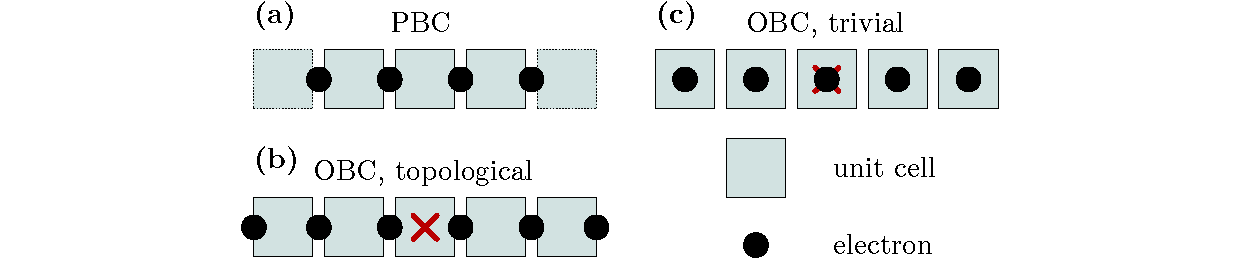
\includegraphics[width=\textwidth]{oal_ssh-fractional.pdf}
\caption[Charge fractionalization in the inversion-symmetric SSH chain]{Charge fractionalization in the inversion-symmetric SSH chain. A red cross marks the center of inversion. \textbf{(a)} For a periodic chain, there is an ambiguity in the choice of the unit cell. On the other hand, with open boundary conditions, the Wannier centers can reside at inequivalent high-symmetry positions in the unit cell. \textbf{(b)} In the topological case, the Wannier centers are located at the unit cell boundary, leading to half charges at the end of an open chain~\cite{Miert16,miertOrtixFractionalCharge17,rhim17}. \textbf{(c)} In contrast, a trivial limit (with no charges) corresponds to the configuration in which the Wannier centers are localized within the unit cell. Note that imposing spectral symmetries is required for realizing a strong topological phase, but this simple picture based on the polarization of a single unit cell cannot distinguish between all the different possible phases.}
\label{fig:ssh-charge}
\end{figure}

In general, the Zak phase can take any value. However, the presence of the spatial inversion $\mathcal{I}$ imposes the constraints on $\gamma_n$ (and therefore on $P_n$). The Berry connection is odd under the action of $\mathcal{I}$, $\bm{\mathcal{A}}_n (-k)  =  -\bm{\mathcal{A}}_n (k)$, which implies $P_n = -P_n \mod |e| a $ and hence
\begin{equation}
P_n =0 \hspace*{0.2cm} \mathrm{or} \hspace*{0.2cm}  P_n = \frac{|e | a}{2} \mod |e| a .
\end{equation}
This is exactly the case of the SSH chain, where the WCCs can be located only at $0$ (that is, at a lattice site) or $a /2$ (between two lattice sites), which we illustrate in Fig.~\ref{fig:ssh-charge}. The latter case corresponds to the topological regime with stronger intercell hoppings, when cutting the system after a full unit cell results in the zero-mode end states. These edge modes carry a fractional charge $|e| /2$. Exactly the same arguments lead to the fractionalization of electrons into Majorana fermions in topological superconductors such as the Kitaev's chain~\cite{Kitaev_2001}.

\section{Boundary phenomenon: corner charges}
\label{sec:corner-ch}
We now move to 2D spinful insulating systems with time-reversal symmetry $\mathcal{T}$ (class AII in the AZ classification, $\mathcal{T}^2 = -1$) and the spatial symmetries corresponding to a symmetry group $\mathcal{G}$. We exclude first-order topological insulators hosting the edge states in co-dimension $1$, so that the models we are studying are generically gapped even in a geometry with open boundary conditions. Additionally, we exclude insulators with bulk (TRS) polarization because those have edge-induced filling anomalies that scale with edge length and therefore result in metallic edges that preclude the existence of stable localized corner charges\cite{benalcazar2018quantization}.

\subsection{Quantization of the corner charge}
\label{sec:bdrychquant}
We assume a tight-binding description of the system of interest and denote by $\mathbf{a}_1$ and $\mathbf{a}_2$ the translation vectors corresponding to the decomposition of the $\mathcal{G}$-symmetric lattice $\Lambda$ into $l$-site unit cells $\mathrm{S} = \{\mathbf{r}_1, \dots, \mathbf{r}_l \}$, where $\mathbf{r}_i$ denotes the position of site $i$ in the unit cell as measured from the unit cell origin $\mathbf{r}_1 \equiv \mathbf{0}$. (Note that here and in the following, we only treat unit cells that are mapped to themselves under all available point-group symmetries, and do not cut through atomic sites. By these properties, a finite-size termination which does not cut through unit cells becomes possible.) We have
\begin{equation}
\Lambda = \bigcup_{x,y \in \mathbb{Z}} \bigcup_{\mathbf{r} \in \mathrm{S}} \left(x \mathbf{a}_1 + y \mathbf{a}_2 + \mathbf{r} \right).
\end{equation}
We are considering tight-binding Hamiltonians of the form
\begin{equation}
\label{eq:tbham}
H = \sum_{\mathbf{v}, \mathbf{w} \in \Lambda} \sum_{\mu,\nu} h_{\mathbf{v} \mu, \mathbf{w} \nu} \, c^\dagger_{\mathbf{v} \mu} c^{\vphantom{\dagger}}_{\mathbf{w} \nu},
\end{equation}
where $\mu,\nu$ run over orbital degrees of freedom defined at each lattice site and $c^\dagger_{\mathbf{v} \mu}$ creates an electron in the orbital $\mu$ at the lattice site $\mathbf{v}$. Hermiticity of $H$ as well as the symmetry requirements posed by $T$ and the symmetry group $\mathcal{G}$ imply some relations among the Hamiltonian elements $h_{\mathbf{v} \mu, \mathbf{w} \nu}$ which we implicitly assume to be fulfilled here and in the following for simplicity.

Given a unit cell decomposition of $\Lambda$ in terms of $S$, we define a \emph{trivial atomic limit} by a Hamiltonian that is adiabatically deformable into one for which the implication
\begin{equation}
\quad \mathbf{v} \in \bigcup_{\mathbf{r} \in \mathrm{S}} \left(x \mathbf{a}_1 + y \mathbf{a}_2 + \mathbf{r} \right) \not\ni \mathbf{w} \quad \Rightarrow \quad h_{\mathbf{v} \mu, \mathbf{w} \nu} = 0
\end{equation}
holds for all choices of $x$ and $y$, that is, there are no couplings between different unit cells.

To calculate corner charges we consider a finite system of $|\mathrm{F}|$ unit cells, via restricting $H$ to a subset $\Lambda_\mathrm{F} \in \Lambda$ (thereby obtaining $H_\mathrm{F}$), which is given by
\begin{equation}
\label{eq:finitelattice}
\Lambda_\mathrm{F} = \bigcup_{x,y \in \mathrm{F}} \bigcup_{\mathbf{r} \in \mathrm{S}} \left(x \mathbf{a}_1 + y \mathbf{a}_2 + \mathbf{r} \right).
\end{equation}
We choose $\Lambda_\mathrm{F}$ so as to retain all point group symmetries contained in $\mathcal{G}$, a subgroup we denote by $\mathcal{G}_\mathrm{F}$ (it does not contain translations or non-symmorphic symmetries). Then we consider a subset $\mathrm{C} \subset \Lambda_\mathrm{F}$ comprised of a minimal (but larger than 1) number of disjoint boundary regions that form an orbit under $\mathcal{G}_\mathrm{F}$ and contain an integer number of unit cells each. We choose $\mathrm{C}$ to cover all boundaries of $\Lambda_\mathrm{F}$. A particular boundary region $\mathrm{c} \subset \mathrm{C}$ has charge
\begin{equation}
\label{eq:bdrychargedef}
Q_\mathrm{c} = \sum_{\mathbf{v} \in \mathrm{c}} \sum_\mu \sum_{l \in \mathrm{occ}} \left|\braket{\mathbf{v} \mu | l}\right|^2,
\end{equation}
where $\ket{l}$ denotes an eigenstate of $H_\mathrm{F}$ that is taken out of the occupied subspace $\mathrm{occ}$ bounded by $E_\mathrm{Fermi}$ and we have $\ket{\mathbf{v} \mu} = c^\dagger_{\mathbf{v} \mu} \ket{0}$ where $\ket{0}$ denotes the electronic vacuum. Since we only consider regions $\mathrm{c}$ that are related to each other by elements of $\mathcal{G}_\mathrm{F}$, they have necessarily the same charge. Now, note that the charge of the full system is an even integer (given by the number of occupied bands $|\mathrm{occ}|$ due to the time reversal symmetry). As long as we choose the regions in $\mathrm{C}$ large enough to ensure that the eigenstates localized in the complement are pure bulk-like in character and unaffected by the presence of a boundary, the charge of the complement of $\mathrm{C}$ is also an even integer. This is always possible when the linear extent by which $\mathrm{C}$ penetrates the bulk is much larger than the correlation length set by the bulk gap. We may then view the states contributing to the charge of the complement of $\mathrm{C}$ as states of a complete system of reduced size that has periodic boundary conditions and even integer charge. We thus deduce that $Q_\mathrm{c}$ is quantized in even integer multiples of $1/q$, where $q = |\mathrm{C}|$ denotes the number of elements in $\mathrm{C}$, that is, disjoint boundary regions. See Figs.~\ref{fig:cornerchargefrac}~(a) and~(b) for an example with threefold rotational symmetry.

\begin{figure}[H]
\centering
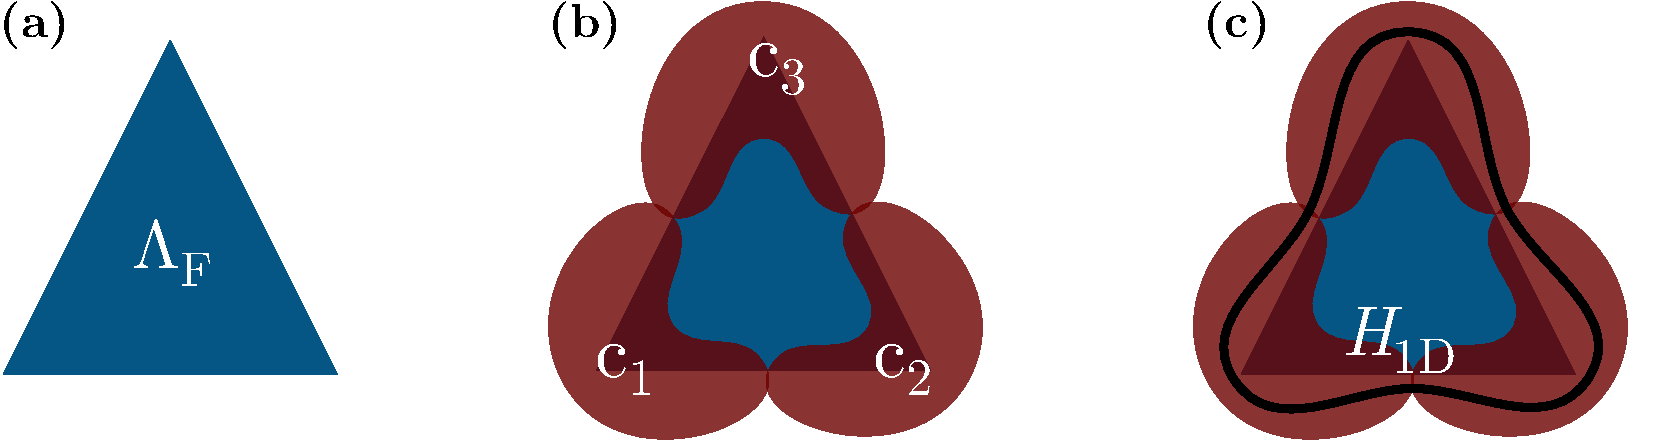
\includegraphics[width=0.85\columnwidth]{oal_charges.pdf}
\caption[Corner charge fractionalization due to $C_3$ rotational symmetry]{Corner charge fractionalization due to $C_3$ rotational symmetry. \textbf({a)} The finite system $\Lambda_\mathrm{F}$ on which $H_\mathrm{F}$ is defined. \textbf{(b)} The boundary regions $\mathrm{c}_1, \mathrm{c}_2, \mathrm{c}_3 \in \mathrm{C}$. Due to the $C_3$ symmetry in $\mathcal{G}_\mathrm{F}$, we have that $Q_{\mathrm{c}_1} = Q_{\mathrm{c}_2} = Q_{\mathrm{c}_3}$. Together with $Q_{\mathrm{c}_1} + Q_{\mathrm{c}_2} + Q_{\mathrm{c}_3} \in 2 \mathbb{Z}$, this implies a corner charge fractionalization in even multiples of $1/3$. \textbf{(c)} A 1D edge addition, modeled by the Hamiltonian $H_{\mathrm{1D}}$. We prove in Section~\ref{sec:bdrychargerobustness} that the corner charges $Q_{\mathrm{c}_i}$ are only changed by even integers.}
\label{fig:cornerchargefrac}
\end{figure}

We call $Q_\mathrm{c}$ the corner charge since, in a pristine OAL, its fractional part derives from exponentially localized Wannier orbitals that are 'cut through' by corners in the boundary of the system~\cite{miertcorners,EzawaWannier19,benalcazar2018quantization}: The Wannier orbitals in OALs are localized at maximal Wyckoff positions in the unit cell, and have shapes that respect the little group of their Wyckoff position. When a Wyckoff position lies on the boundary of the unit cell, the boundary cuts through the respective Wannier orbital. The corner charge $Q_\mathrm{c}$ can then be calculated conveniently and is equal to the volume that all occupied Wannier functions integrate to in $\mathrm{c}$ (where a single Wannier function is normalized to unit volume).

Any trivial atomic limit has $Q_\mathrm{c} \in 2\mathbb{Z}$ for any such choice of boundary region: when different unit cells are not coupled to each other, the charge in each unit cell has to be equal to the total charge of the occupied subspace of $H_{\mathrm{F} = \{(0,0)\}}$, which is necessarily an even integer. We may then define \emph{corner charge fractionalization} as occurring in systems for which $Q_\mathrm{c} \mod 2$ is equal to non-zero even integer multiples of $1/q$ (odd integer multiples are forbidden by TRS). Note that we assume all systems with non-trivial corner charge to be given by OALs, which have a representation in terms of exponentially localized Wannier functions~\cite{MarziariWF2012, Bradlyn17}. However, the corner charge formulas we supply in Section~\ref{sec:mappingformulae} apply equally well to fragile phases~\cite{PhysRevLett.121.126402,BarryFragile,KoreanTBG,wieder2018axion,MaiaFragile1,MaiaFragile2,MaiaFragile3}. These can always be adiabatically continued into OALs when other OALs are added. For a calculation of the corner charge in spinful materials, such a 'trivialization' of a fragile phase becomes necessary only in the symmetry class that has $C_4$ rotational symmetry as its sole crystalline component, since this symmetry does not by itself allow for explicit corner charge formulas in terms of the elementary topological invariants we consider. The classification of corner charge fractionalization in class AII and symmetry group $\mathcal{G}$ is given by the set of inequivalent $Q_\mathrm{c} \mod 2$ that cannot be changed without breaking $\mathcal{G}_\mathrm{F}$ or closing the bulk gap. Since any finite-size geometry breaks the remaining non-symmorphic symmetries a system might have, we do not need to consider their effect on charge fractionalization. 

\begin{figure}[H]
\centering
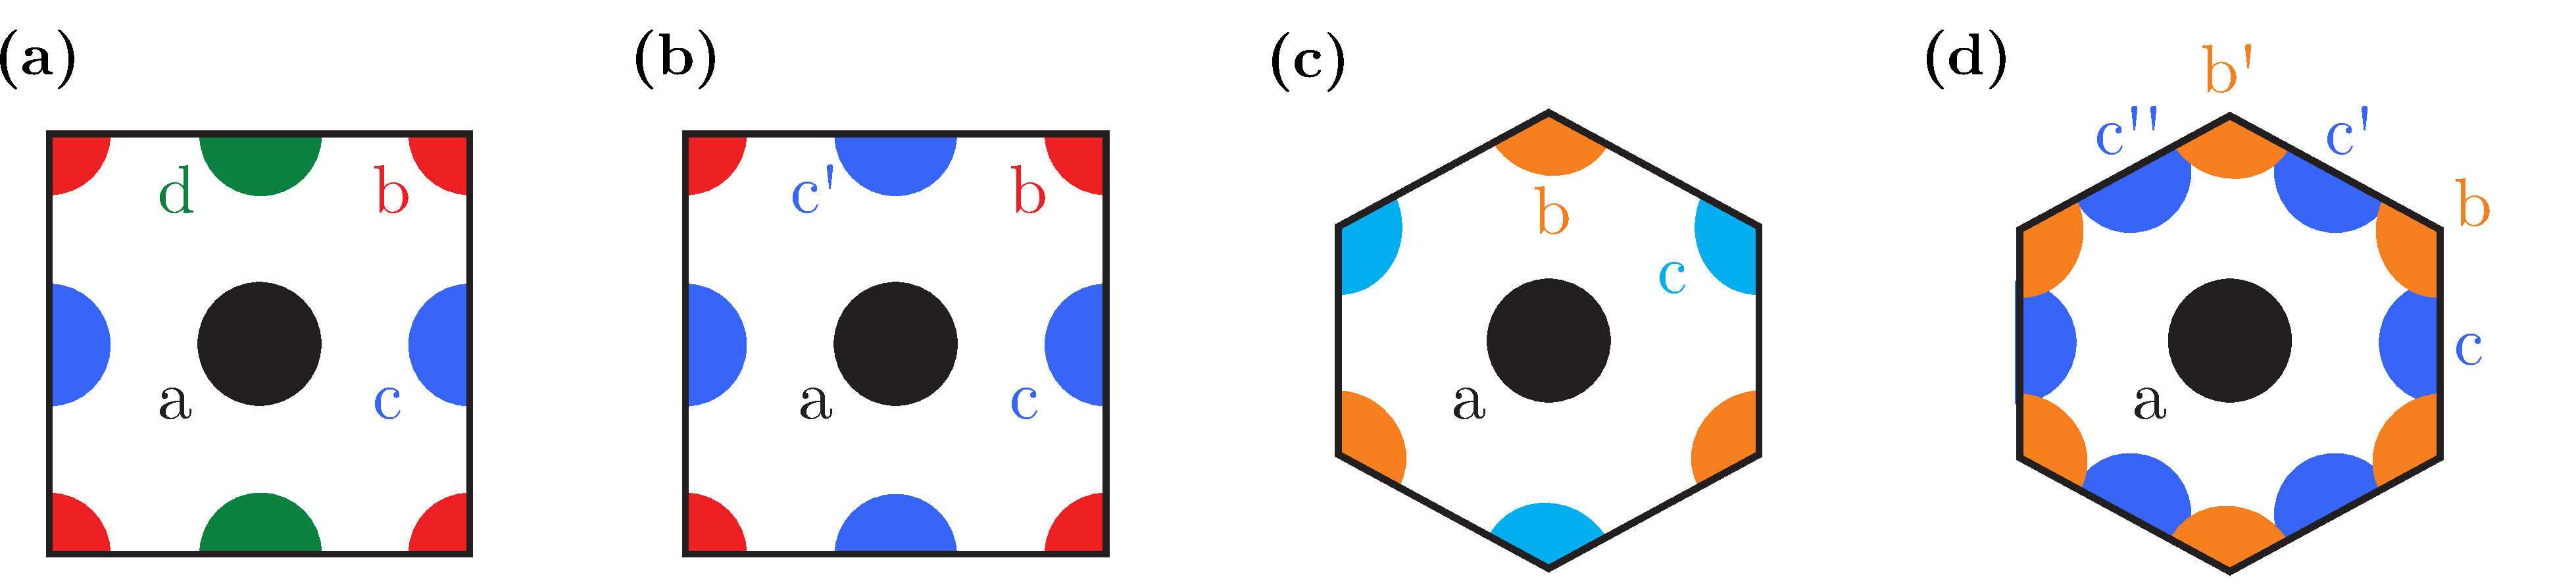
\includegraphics[width=\textwidth]{oal_wyckoff.pdf}
\caption[Maximal Wyckoff positions for unit cells with rotational symmetry]{Maximal Wyckoff positions for unit cells with rotational symmetry. \textbf{(a)} $C_2$ symmetry. \textbf{(b)} $C_4$ symmetry. \textbf{(c)} $C_3$ symmetry. \textbf{(d)} $C_6$ symmetry or $C_3 + \mathcal{I}$ symmetry. Boundary charges arise when the Wyckoff positions which Wannier centers are located at are cut through by the crystal termination.}
\label{fig:wyckpositions}
\end{figure}

\subsection{Stability of the corner charge}
\label{sec:bdrychargerobustness}
We now discuss to what extent symmetry-preserving edge manipulations can change the corner charge $Q_\mathrm{c}$ defined in Eq.~\eqref{eq:bdrychargedef}. We treat an edge manipulation as the introduction of an additional 1D system along the circumference of the finite 2D sample, and ask how the corner charges of the combined system, defined on the appropriately augmented Hilbert space, can differ from those of the original 2D model. Since charges are additive it is enough to determine the possible charges of the 1D system. In the following, we take $Q$ to be the total charge of the 1D addition. It is even due to the requirement that we may only add complete and non-anomalous gapped 1D systems with TRS. We then use the remaining crystalline symmetries to derive further constraints on the charges $Q_{\mathrm{c}}$ that the 1D system contributes to a boundary region $\mathrm{c}$.

We note that the point group symmetries in 2D that $\mathcal{G}_\mathrm{F}$ can contain are mirror and $n$-fold rotational symmetries, where $n \in \{2,3,4,6\}$. We first discuss the latter case of $C_n$ rotational symmetries. For spinful systems with TRS, we have $(C_n)^n = -1$. Let $H_{\mathrm{1D}}$ denote a general 1D TRS gapped Hamiltonian defined on a Hilbert space of $L$ lattice sites (with $L/n$ an integer), possibly augmented by orbital degrees of freedom (see also Fig.~\ref{fig:cornerchargefrac}~(c)). A $C_n$ rotational symmetry
\begin{equation}
C_n H_{\mathrm{1D}} C_n^\dagger = H_{\mathrm{1D}},
\end{equation}
implies that we can choose the order of regions $\mathrm{c}_i \in \mathrm{C}$ (which in combination cover all of the $L$ sites of the 1D system) such that in real space the symmetry effects $\mathrm{c}_i \rightarrow \mathrm{c}_{i+1 \mod n}$, that is, a translation by $L/n$ sites. Now, due to $(C_n)^n = -1$, rotations are equivalent to translations around a 1D circle that encloses a $\pi$-flux. Let $t$ be the operator for translations by a single site, \ie, it shifts site $r \in \{1,\dots,L\}$ of the 1D lattice to site $r+1 \mod L$. It is not a symmetry of $H_{\mathrm{1D}}$, however, we can obtain a $t$-symmetric Hamiltonian (on a ring enclosing a $\pi$-flux) by adding up $L/n$ copies of $H_{\mathrm{1D}}$ that are subsequently shifted by one lattice site, to arrive at
\begin{equation}
H_{\mathrm{1D}}^{\mathrm{TRN}} = H_{\mathrm{1D}} \oplus t H_{\mathrm{1D}} t^\dagger \oplus \dots \oplus t^{L/n-1} H_{\mathrm{1D}} (t^\dagger)^{L/n-1},
\end{equation}
which acts on an $L/n$-fold enlarged Hilbert space. The occupied subspace of $H_{\mathrm{1D}}^{\mathrm{TRN}}$ has a total charge of $Q L/n$ and enjoys a translational symmetry that corresponds to $L$ repeated unit cells, with twisted boundary conditions so as to accommodate the $\pi$-flux. It is gapped and has TRS just as $H_{\mathrm{1D}}$, and its charge thus necessarily corresponds to an even integer number of filled Bloch bands, which each hold $L$ states. We conclude that its charge per unit cell $Q/n$ is an even integer. Returning our attention to $H_{\mathrm{1D}}$, since all boundaries $\mathrm{c}$ carry the same charge, this is exactly the corner charge $Q_{\mathrm{c}} = Q/n$. Thus in the case of $C_n$-symmetries there is no 1D addition that can trivialize the fractional corner charges of a 2D OAL.

Next, we turn to mirror symmetries, which for spinful systems satisfy $\mathcal{M}^2 = -1$. In the case of two reflections, say $\mathcal{M}_x$ and $\mathcal{M}_y$, we also have a two-fold rotation symmetry $C_2 = \mathcal{M}_x \mathcal{M}_y$, which by the argument above allows us to conclude that all corner charges $Q_{\mathrm{c}}$ contributed by any gapped and TRS 1D addition are necessarily even (note that the minimal non-trivial boundary decomposition has $q = 2$). When there is only a single mirror symmetry, we cannot argue along these lines, since it does not act on the 1D real space as a translation. In fact, it 'translates' different sites along the 1D chain by different amounts. Hence, here the symmetry constraint on $Q_{\mathrm{c}}$ is the same as that for the 2D bulk, namely that $Q_{\mathrm{c}_i} \in \mathbb{Z}$, $i=1,2$, (compare this to the $Q_{\mathrm{c}_i} \in 2\mathbb{Z}$ we obtain for $C_2$ symmetry) and a fractional charge of $1 \mod 2$ can be trivialized. With a single mirror symmetry, the charges are not robust.

Finally, we note that in the case where we have $C_3$ symmetry as well as 3D inversion symmetry $\mathcal{I}$ (which is the same as $C_2 M_z$ symmetry), we can define an effective $1/6$ translation by $t_{1/6} = \mathcal{I} C_3^2$ which allows to argue that patches $\mathrm{c}$ of size $1/6$ of the linear extent of the full 1D system have even integer charge. This is important for the robustness of the $Q_\mathrm{c} = 1/6$ corner charges of this symmetry class. Since any finite-size geometry breaks the remaining non-symmorphic symmetries a system might have, we do not need to consider their effect on charge fractionalization. We conclude that quantized corner charges can be changed by 1D edge manipulations only in the case of a single mirror symmetry.

\section{Bulk indices}
\label{sec:topologicalindices}
To identify different EBRs, we employ a combination of symmetry indicator~\cite{Hughes:inv,PhysRevB.86.115112, Slager2013,benalcazar2014,Po2017, Bradlyn17,SongZhang17,Khalaf17,benalcazar2018quantization} and Wilson loop~\cite{WilczekZee,berry84,ZakPhase1,ZakPhase2,Slager2013,PhysRevB.89.155114, Slager17,BarryFragile} topological invariants. These can be evaluated from the crystal's Bloch Hamiltonian $\mathcal{H}(\mathbf{k})$ and so do not require a real-space calculation to be performed. The main ingredient for both kinds of invariants is the bundle of occupied Bloch states $\ket{u_{m}(\mathbf{k})}$. Here, $\mathbf{k}$ is an element of the first Brillouin zone of the crystal.

\begin{figure}[H]
\centering
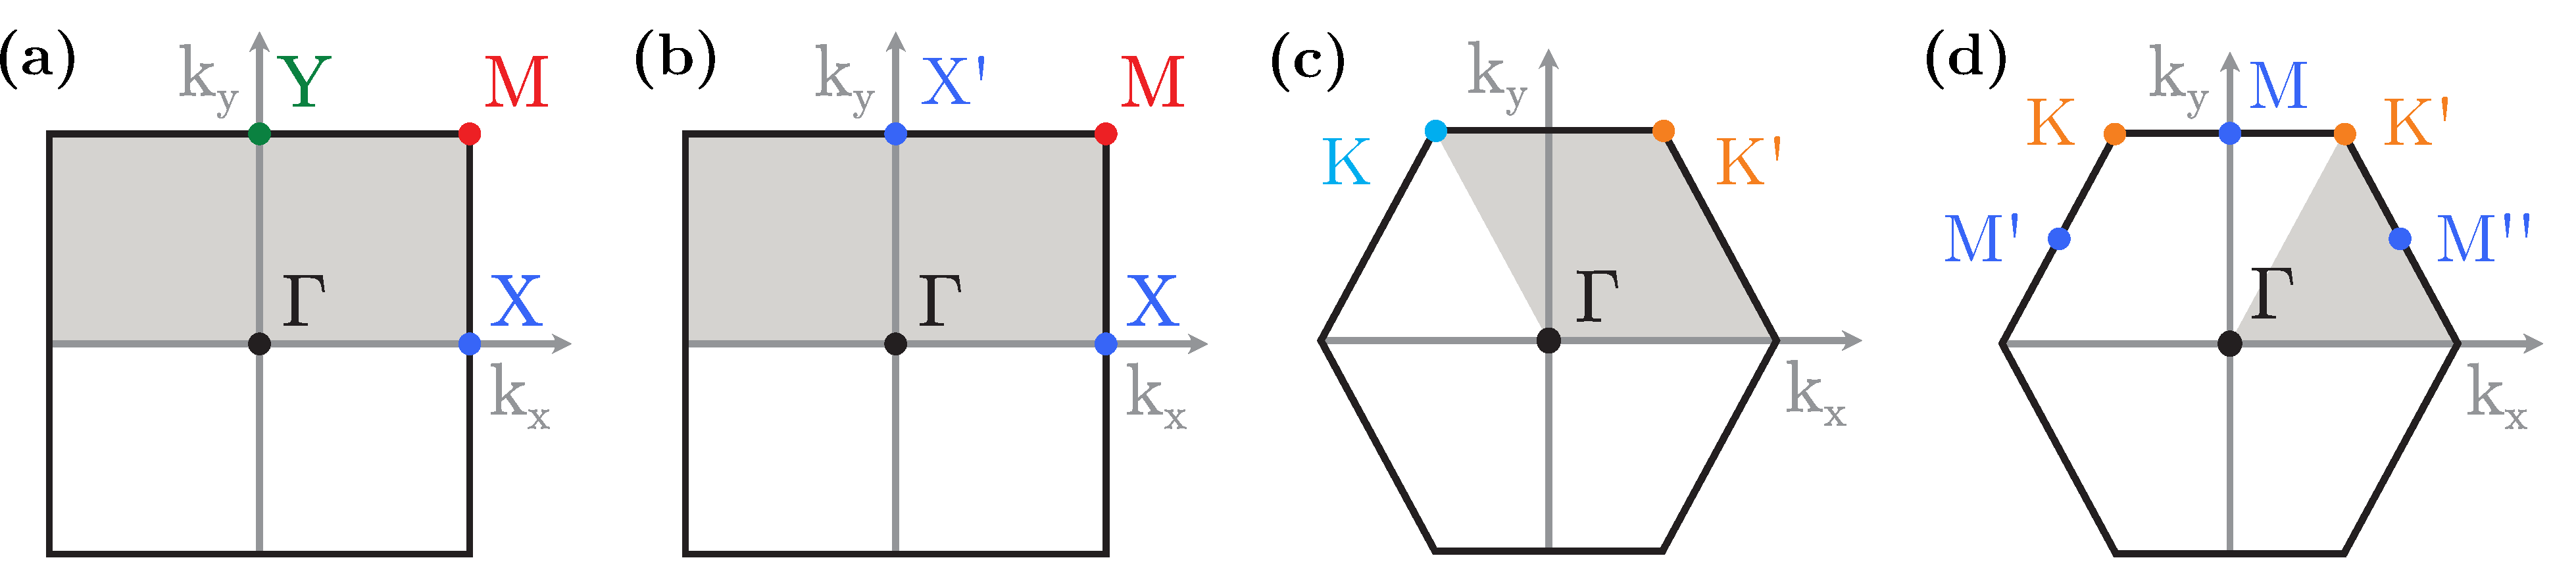
\includegraphics[width=0.95\textwidth]{oal_bz.pdf}
\caption[Brillouin zones of crystals with $C_2$, $C_4$, $C_3$, and $C_6$ symmetries and their rotation invariant points]{Brillouin zones of crystals with $C_2$, $C_4$, $C_3$, and $C_6$ symmetries and their rotation invariant points. In $C_2$-symmetric systems there are three 2-fold HSPs: $\mathbf{X}$, $\mathbf{Y}$, and $\mathbf{M}$. In $C_4$-symmetric systems there are two 2-fold HSPs: $\mathbf{X}$ and $\mathbf{X'}$, and one 4-fold HSP: $\mathbf{M}$. In $C_3$-symmetric systems there are only two 3-fold HSPs: $\mathbf{K}$ and $\mathbf{K'}$. Finally, in $C_6$-symmetric systems there are three 2-fold HSPs: $\mathbf{M}$, $\mathbf{M'}$, and $\mathbf{M''}$, as well as two 3-fold HSPs: $\mathbf{K}$ and $\mathbf{K'}$.}
\label{fig:BZ}
\end{figure}

\subsection{Symmetry indicators}
The Fu-Kane parity criterion for the inversion-symmetric TIs~\cite{FuKane2007} that we introduced in the Chapter~\ref{ch:topo-intro} is in fact the first instance of a more general framework for symmetry indicators. The symmetry-based methods allow for an efficient diagnosis and characterization of the band structures as they require only symmetry representations of the Bloch states at HSPs~\cite{Bradlyn17, Po2017}. Consider a unitary crystal symmetry $\mathcal{S}$ that is realized on the Bloch Hamiltonian as $\mathcal{S} \mathcal{H}(\mathbf{k}) \mathcal{S}^\dagger = \mathcal{H}(\mathsf{S} \mathbf{k})$ and acts on the momenta as $\mathbf{k} \rightarrow \mathsf{S} \mathbf{k}$. We can then calculate its corresponding symmetry indicator topological invariants from the eigenvalues of the matrices
\begin{equation}
S_{mn} = \bra{u_m(\mathbf{\bar{k}})} \mathcal{S} \ket{u_n(\mathbf{\bar{k}})},
\end{equation}
where $m,n$ run over the occupied subspace only and $\mathbf{\bar{k}} = \mathsf{S} \mathbf{\bar{k}}$ are high-symmetry points (HSPs) of the Brillouin zone that are left invariant by the symmetry $\mathcal{S}$ (see also Fig.~\ref{fig:BZ}). An $n$-fold symmetry acting on spinful fermions satisfies $\mathcal{S}^n = \pm1$ (positive sign for 3D inversion, negative sign for 2D mirror and rotational symmetries), this, together with TRS, imposes constraints on the possible eigenvalues of $S_{mn}$ and allows for the definition of topological invariants that capture the different symmetry representations of the occupied bands across the BZ. A trivial atomic limit, being deformable to a momentum-independent Hamiltonian, will have the same representation across HSPs that are invariant under the same symmetry and hence will have trivial symmetry indicator invariants. Non-trivial symmetry indicator invariants, on the other hand, indicate that the bands adopt different representations of the symmetry across the BZ and correspond to OALs.

\subsection{Wilson loops}
The Wilson loop (along a closed, non-contractible path $\gamma$ in the BZ that starts and ends at the momentum $\mathbf{k}^*$) is an operator on the filled band subspace of $\mathcal{H}(\mathbf{k})$ defined as
\begin{equation}
W_\gamma = \prod_{\mathbf{k}}^{\gamma} P(\mathbf{k}),
\label{eq:wilson-gen}
\end{equation}
where $P(\mathbf{k})= \sum_{m \in \mathrm{occ}} \ket{u_m(\mathbf{k})}\bra{u_m(\mathbf{k})}$ is the projector onto the subspace of filled bands at momentum $\mathbf{k}$. Note that we choose a gauge where $\mathcal{H}(\mathbf{k}) = \mathcal{H}(\mathbf{k}+\mathbf{G})$ for a reciprocal lattice vector $\mathbf{G}$ and the product is path-ordered along $\gamma$. For numerical purposes, the Wilson loop in Eq.~\eqref{eq:wilson-gen} can be discretized as
\begin{equation}
\begin{aligned}
[W_\gamma]_{mn} &= \braket{ u_{m, (k_1, \mathbf{k}^*) } | \prod_{k_2}^{\mathbf{k}^* \leftarrow \mathbf{k}^*} P(k_1, k_2) | u_{n, (k_1, \mathbf{k}^*) }}; \\
\mathrm{with} \hspace*{0.5cm }\prod_{k_2}^{\mathbf{k}^* \leftarrow \mathbf{k}^*} P(k_1, k_2) &= \lim_{\Delta \rightarrow 0} P(k_1, \mathbf{k}^*) P(k_1, \mathbf{k}^* - \Delta) \ldots P(k_1, \Delta) P(k_1, \mathbf{k}^*),
\end{aligned}
\end{equation}
where $k_1, k_2$ are momenta along the path $\gamma$. The Wilson loop operator satisfies $W_\gamma W_\gamma^\dagger = P(\mathbf{k}^*)$. Since any projector fulfils $[P(\mathbf{k})]^2 = P(\mathbf{k})$, \ie is idempotent, its eigenvalues are either zero or of the form $e^{\mathrm{i} \theta_\alpha^\gamma}$, $\alpha = 1 \dots N$. In the following, we refer to the set of $\{\theta_\alpha^\gamma\}_{\alpha = 1 \dots N}$ as the Wilson loop spectrum (which is gauge-invariant), suppressing the zero eigenvalues. Note that the $\theta$'s phases are only defined modulo $2 \pi$. The eigenvalues of the Wilson loop are related to the spectrum of the band-projected position operator $P (\mathbf{k}) x P (\mathbf{k})$ or, equivalently, to the centers of hybrid Wannier functions, which are exponentially localized in the one direction and completely delocalized in the remaining directions~\cite{PhysRevB.89.155114}.

The antiunitary TRS $\mathcal{T}$ acts on the Bloch Hamiltonian as $\mathcal{T} \mathcal{H}(\mathbf{k}) \mathcal{T}^{-1} = \mathcal{H}(-\mathbf{k})$. For the projectors this implies $\mathcal{T} P(\mathbf{k}) \mathcal{T}^{-1} = P(-\mathbf{k})$. When $\gamma$ is mapped onto itself by TRS, and its starting point satisfies $\mathbf{k}^* = -\mathbf{k}^*$ up to a reciprocal lattice vector, we then have 
\begin{equation}
\label{eq:TRSonWilson}
\mathcal{T} W_\gamma \mathcal{T}^\dagger = \prod_{\mathbf{k}}^{\gamma} P(-\mathbf{k}) = W_\gamma^\dagger.
\end{equation}
Due to $\mathcal{T}$ being antiunitary and $\mathcal{T}^2 = -1$, this implies a Kramers degeneracy of the Wilson loop spectrum, \ie, every $\theta_\alpha^\gamma$ is (at least) two-fold degenerate when $\gamma$ is mapped onto itself by time reversal.

Now, if there is a crystal symmetry $\mathcal{S}$ that reverses the direction of $\gamma$ and leaves the starting point invariant so that $\mathbf{k}^* = \mathsf{S} \mathbf{k}^*$ up to a reciprocal lattice vector, we have 
\begin{equation}
\label{eq:reflectiononWilson}
\mathcal{S} W_\gamma \mathcal{S}^\dagger =  \prod_{\mathbf{k}}^{\gamma} \left[\mathcal{S} P(\mathbf{k}) \mathcal{S}^\dagger \right]
= W_\gamma^\dagger.
\end{equation}
Since $\mathcal{S}$ is unitary, the Wilson loop is unitarily equivalent to its complex conjugate and so its eigenvalues come in complex conjugated pairs. This implies a symmetry of the Wilson loop spectrum around $\theta=0$, for every $\theta_\alpha^\gamma$ there is a corresponding $-\theta_\alpha^\gamma \mod 2\pi$.

\subsubsection{Nested Wilson loops}
We may furthermore employ nested Wilson loops~\cite{BABHughesBenalcazar17,Benalcazar17}. Let $W_i (k_j)$, $i \neq j$, denote the Wilson loop along the non-contractible loop $\gamma: (k_i = 0, k_j) \rightarrow (k_i = 2\pi, k_j)$, where ($k_i$, $k_j$) labels a point in the two-dimensional BZ in some basis (chosen such that $k_{i,j} = 0$ and $k_{i,j} = 2\pi$ are related by reciprocal lattice vectors). Consider the Wilson loop Hamiltonian $H_{W_i} (k_j)$, defined by
\begin{equation}
\left[e^{\mathrm{i} H_{W_i}(k_j)} \right]_{mn}= \bra{u_m(k_i=0,k_j)} W_i (k_j) \ket{u_n(k_i=0,k_j)}.
\end{equation}
Equations~\eqref{eq:TRSonWilson} and~\eqref{eq:reflectiononWilson} then imply
\begin{equation}
\begin{aligned}
\mathcal{T}_{k_j} H_{W_i} (k_j) \mathcal{T}_{k_j}^\dagger &= H_{W_i} (-k_j), \\
\mathcal{S}_{k_j} H_{W_i} (k_j) \mathcal{S}_{k_j}^\dagger &= - H_{W_i} (\mathsf{S} k_j),
\end{aligned}
\label{eq:nestedWilsonprops}
\end{equation}
where we defined
\begin{equation}
\begin{aligned}
\left(\mathcal{T}_{k_j} \right)_{mn} &= \bra{u_m(-k_j)} \mathcal{T} \ket{u_n(k_j)}, \\
\left(\mathcal{S}_{k_j} \right)_{mn} &= \bra{u_m(\mathsf{S}k_j)} \mathcal{S} \ket{u_n(k_j)}.
\end{aligned}
\end{equation}
We see that $\mathcal{T}$ implies a TRS of the Wilson loop Hamiltonian, whereas $\mathcal{S}$ implies a particle-hole symmetry. These properties are needed for the definition of quantized topological invariants of the \emph{nested Wilson loop}: We define $W_i^\mathrm{b}$ as the Wilson loop calculated from a gapped set of eigenstates $\mathrm{b}$ of $H_{W_i} (k_j)$ along a closed, non-contractible path $k_j: 0 \rightarrow 2\pi$ in the reduced BZ.

We differentiate between three kinds of nested Wilson loops that differ by the choice of the set of eigenstates $\mathrm{b}$: (1) The nested loop $W_i^0$, which is calculated from the two bands in the spectrum of $H_{W_i} (k_j)$ that at $k_j = 0, \pi$ have a degeneracy pinned to the Wilson eigenvalue $0$ (note that any such degeneracy at $k_j = 0$ implies one at $k_j = \pi$ and vice versa due to the absence of Wannier center flow in (obstructed) atomic limits). (2) The nested Wilson loop $W_i^{\lambda}$, calculated for the upper \emph{or} lower half of the bands in the spectrum of $H_{W_i} (k_j)$ that are \emph{not} pinned at $k_j = 0, \pi$ to a Wilson eigenvalue $0,\pi$ (that is, half of the freely dangling Wilson bands, which by the particle hole symmetry come in pairs). (3) The nested loop $W_i^{\pi}$, which is calculated from the two bands in the spectrum of $H_{W_i} (k_j)$ that at $k_j = 0, \pi$ have a degeneracy pinned to the Wilson eigenvalue $\pi$.

The nested Wilson loops of type (1) and (3) cannot be trivialized by transformations that preserve $\mathcal{S}$ and $\mathcal{T}$ and are adiabatic with respect to the bulk gap. The reason is that the invariants calculated from these loops are equal to the partial polarizations of Wilson bands pinned to eigenvalues $0$ or $\pi$ by $\mathcal{S}$ at the transverse momenta $k_j = 0, \pi$. Wilson gap closings that preserve the energy gap can only occur in pairs (due to $\mathcal{S}$) at intermediate transverse momenta $k_j, -k_j$. It is rigorously shown in Appendix A of Ref.~\cite{Sander2DTCI2019} that these gap closings together always contribute integer multiples of $2\pi$ to the nested partial polarization, and therefore cannot trivialize Wilson loops of type (1) and (3). Here, we do not consider invariants derived from Wilson loops of type (2).

\section{Classification with respect to $C_n$ and inversion symmetries}
\label{sec:class-symm}
We now list the topological invariants that can be defined for a given point group. We find that often the inclusion of the $\mathcal{I}$ symmetry allows for the replacement of Wilson-loop invariants by symmetry indicator invariants. For the discussion of symmetry indicators, we make use of the definitions and derivations presented in Sections~\ref{sec:rotsymwladimir} and~\ref{sec:inductionEBRs} of the Appendix. Note that in the following, and as motivated at the beginning of Section~\ref{sec:corner-ch}, we explicitly exclude invariants that characterize topological insulators because they are necessarily gapless along the edges in a 2D geometry with open boundary conditions, and so do not allow for stable quantized corner charges. In addition to removing some invariants from our analysis altogether, this imposes constraints on the Wilson loops.

As shown in Section~\ref{sec:bdrychargerobustness}, mirror symmetries can protect fractional corner charges only when they are combined to yield a twofold rotational symmetry. The protecting symmetries we consider are therefore $C_n$ rotations, with or without an additional 3D inversion symmetry $\mathcal{I}$. The inclusion of the $\mathcal{I}$ symmetry allows us to extend our discussion to the experimentally relevant case of 2D honeycomb monolayers with non-zero buckling. We note that inversion effectively replaces $C_2$ in its role of enforcing a $Q_\mathrm{c} = 0,1\mod 2$ quantization of the corner charge, but due to $\mathcal{I}^2 = +1$ (whereas $(C_2)^2 = -1$) allows for symmetry indicator invariants. Furthermore, in the case of $C_4$ symmetry, we find that we require an additional inversion symmetry in order to be able to read off the corner charge from the available topological invariants. Inversion symmetry is however, unlike $C_4$, not necessary for the topological robustness of the corner charge.

\begin{figure}[H]
\centering
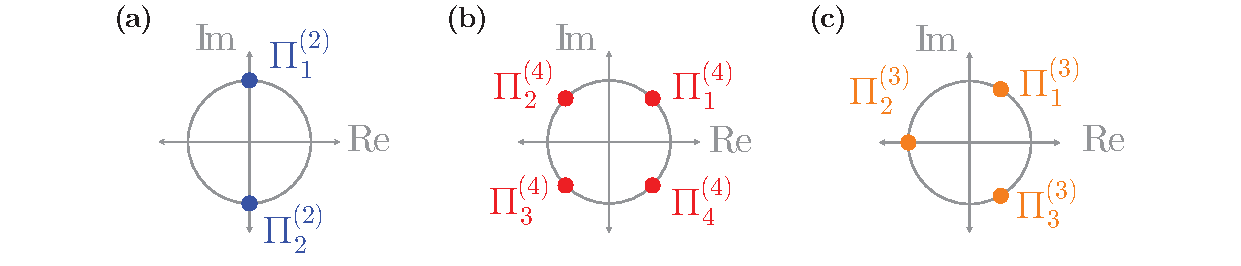
\includegraphics[width=0.95\textwidth]{oal_evals.pdf}
\caption[Sets of allowed eigenvalues for spinful rotational symmetries]{Sets of allowed eigenvalues for spinful rotational symmetries. \textbf{(a)} $C_2$ symmetry. \textbf{(b)} $C_4$ symmetry. \textbf({c)} $C_3$ symmetry. The possible eigenvalues of $C_6$ symmetry are not shown, since they do not allow for the definition of symmetry indicators (there is at most one $C_6$-symmetric point in any two-dimensional Brillouin zone).}
\label{fig:eigvalsets}
\end{figure}

We emphasize that our list of invariants may not be exhaustive. As noted in Ref.~\cite{BarryFragile}, it is in general difficult to identify all possibly non-trivial Wilson loop invariants. We only treat 'straight' (nested) Wilson loops, which for a given a starting point go around one of the two inequivalent non-contractible loops of the Brillouin zone torus.

\subsection{$C_2$ symmetry}
\subsubsection*{Symmetry indicator invariants} 
The BZ has four HSPs, see Fig.~\ref{fig:BZ}~(a). All the points are invariant under $C_2$. Thus, they all have $C_2$ eigenvalues ${+\mathrm{i},-\mathrm{i}}$ (consult Fig.~\ref{fig:eigvalsets}~(a)). However, since all the HSPs are also time-reversal invariant momenta, the eigenvalues have to come in complex-conjugate pairs, leading to a single available 2D irreducible representation. Therefore, the $C_2$ eigenvalues do not distinct different topological phases and there are no symmetry indicator invariants.

\subsubsection*{Wilson-loop invariants} 
For every closed high-symmetry line $\gamma$ (which connects two HSPs) of the 2D BZ that is left invariant by $C_2$, we can define a Wilson loop that is TRS and $C_2$ symmetric. Due to Eqs.~\eqref{eq:TRSonWilson} and~\eqref{eq:reflectiononWilson}, the parities of the numbers of $\theta_\alpha^\gamma = 0$ and $\theta_\alpha^\gamma = \pi$ eigenvalues in its spectrum cannot be changed under adiabatic deformations of $\mathcal{H}(\mathbf{k})$: adiabatic perturbations of the Hamiltonian at most move eigenvalues in or out of $0$ (resp. $\pi$) in pairs due to the Kramers symetry induced by particle-hole symmetry. A topological invariant of $W_\gamma$ with spectrum $\{\theta_\alpha^\gamma\}_{\alpha = 1 \dots N}$ is therefore given by
\begin{equation}
\label{eq:wilsonloopwithreflectioninvariant}
\nu_{\gamma} = -\frac{\mathrm{i}}{\pi} \log \left( \prod_{\alpha=1,3,\dots,N-1} e^{\mathrm{i} \theta_\alpha^\gamma} \right) \mod 2,
\end{equation}
where the product is taken over only one eigenvalue of each Wilson loop Kramers pair. We call $\nu_{\gamma} = 0$ trivial and $\nu_{\gamma} = 1$ non-trivial. This invariant is equivalent to the TRS polarization~\cite{MirrorInsulatorOrtix} and counts the parity number of Wilson loop pairs of eigenvalues equal to $\pi$. We also define
\begin{equation}
\label{eq:wilsonloopwithreflectioninvariant2}
\mu_{\gamma} = -\frac{\mathrm{i}}{\pi} \log \left( \prod_{\alpha=1,3,\dots,N-1} e^{\mathrm{i} (\pi-\theta_\alpha^\gamma)} \right) \mod 2,
\end{equation}
which counts the number of Wilson loop pairs of eigenvalues equal to $0$. The invariants $\nu_{\gamma}$ and $\mu_{\gamma}$ are not independent when the total number of bands $N$ is fixed. They obey
\begin{equation}
\mu_{\gamma} = \nu_{\gamma} + \frac{N}{2} \mod 2.
\end{equation}
Therefore, we drop $\mu_\gamma$ as it provides redundant topological information. In the following, we consider Wilson loops that go through high-symmetry points in the 2D BZ. We denote by $\nu_{\mathbf{A B}}$ the loop that goes from point $\mathbf{A}$ to point $\mathbf{B}$ and then back to $\mathbf{A}$ via the shortest non-contractible loop around the BZ torus.

There are in total four TRIMs and three topologically inequivalent straight and $C_2$-symmetric Wilson loops. This can be seen by noting that, holding one of the four $C_2$-symmetric momenta fixed as a starting point, there are two incontractible loops around the Brillouin zone torus (which necessarily go through one other $C_2$-symmetric momentum). Keeping in mind that path-reversed Wilson loops are not independent (as per Eq.~\eqref{eq:reflectiononWilson}), this naively yields the set of Wilson loop invariants $\{\nu_{\mathbf{\Gamma X}}, \nu_{\mathbf{\Gamma Y}}, \nu_{\mathbf{X M}}, \nu_{\mathbf{Y M}}\}$. We note however that the path denoted by $\mathbf{Y \Gamma} - \mathbf{\Gamma X} - \mathbf{XM}$ is topologically equivalent to the path denoted by $\mathbf{Y M}$ and so we have
\begin{equation}
\nu_{\mathbf{Y M}} = \nu_{\mathbf{\Gamma Y}} \nu_{\mathbf{\Gamma X}} \nu_{\mathbf{X M}}.
\end{equation}
The remaining invariants are further constrained due to the requirement that the $\mathbb{Z}_2$ TI invariant $\Delta_{\mathrm{TI}}$ vanishes: we have that
\begin{equation}
\begin{aligned}
\Delta_{\mathrm{TI}} & = \nu_{\mathbf{\Gamma X}} + \nu_{\mathbf{Y M}} \mod 2 \\
& = \nu_{\mathbf{\Gamma Y}} + \nu_{\mathbf{X M}} \mod 2.
\end{aligned}
\end{equation}
We are left with two Wilson loop invariants.

Similarly, we may define the quantized invariants $\nu_{x,y}^{0,\pi}$ and $\mu_{x,y}^{0,\pi}$ from the nested Wilson loops $W_{x,y}^{0,\pi}$, since these are calculated for particle-hole symmetric sets of bands~\cite{BenMoTe2,wieder2018axion} (in contrast to $W_{x,y}^{\lambda}$, which does not satisfy Eq.~\eqref{eq:nestedWilsonprops}): the anti-commutativity with the Wilson loop Hamiltonian that distinguishes particle-hole symmetry from a reflection symmetry is irrelevant from the point of view of the nested Wilson loop, as long as the latter is defined via a projector onto a particle-hole symmetric set of bands. We may therefore define $\nu_{x,y}^{0,\pi}$ and $\mu_{x,y}^{0,\pi}$ just as in Eqs.~\eqref{eq:wilsonloopwithreflectioninvariant} and~\eqref{eq:wilsonloopwithreflectioninvariant2}, where $\theta_\alpha^\gamma$ this time refers to the spectrum of the nested Wilson loop. As before, we drop the $\mu$ invariants since they are not independent when the number of occupied Wilson bands is held fixed. Taking into account the constraints~\cite{Sander2DTCI2019} 
\begin{equation}
\begin{aligned}
\nu_{x}^{0} + \nu_{x}^{\pi} & \mod 2 = \nu_{\mathbf{\Gamma Y}}, \\
\nu_{y}^{0} + \nu_{y}^{\pi} & \mod 2 = \nu_{\mathbf{\Gamma X}}, \\
\nu_{x}^{\pi} &= \nu_{y}^{\pi},
\end{aligned}
\end{equation}
reduces the number of independent invariants to three. The third equation can be seen in the following way: $\nu_{x}^{\pi}$ is non-zero if and only if the occupied subspace hosts an odd number of Wannier-Kramers pairs whose centers are shifted by $1/2$ in both $x$ and $y$ direction (taking the lattice constant to be $1$) with respect to the center of the unit cell, \ie, if there is an odd number of Kramers pairs at Wyckoff position $1b$ of the crystal (see also Table~\ref{tab:EBRc2}). This Wyckoff position stays unchanged when exchanging $x$ and $y$, we therefore obtain that $\nu_{x}^{\pi}$ is non-zero if and only if $\nu_{y}^{\pi}$ is non-zero. Note that the corresponding statement does not hold for $\nu_{x}^{0}$ and $\nu_{y}^{0}$, since these indicate Wannier-Kramers pairs at the $1c$ and $1d$ Wyckoff positions, respectively. We therefore choose the classification to be given by
\begin{equation} 
\begin{aligned}
\chi^{(2)} = \{\nu_{\mathbf{\Gamma X}},\nu_{\mathbf{\Gamma Y}}, \nu_{x}^{\pi}\}.
 \end{aligned} 
 \label{eq:c2classificationWithoutInversion}
 \end{equation}

\subsubsection*{With inversion symmetry}
$C_2 + \mathcal{I}$ symmetry is equivalent to $\mathcal{I}$ symmetry for all our purposes. Inversion symmetry allows us to replace the $\mathbb{Z}_2$ valued Wilson-loop invariants by $2\mathbb{Z}$-valued symmetry indicators. The BZ has the $\mathcal{I}$-invariant points $\mathbf{\Gamma}$, $\mathbf{X}$, $\mathbf{Y}$ and $\mathbf{M}$, which support the six inversion eigenvalue invariants
\begin{equation}
\begin{aligned}
[X^\mathcal{I}_i]&= \#X^\mathcal{I}_i - \#\Gamma^{\mathcal{I}}_i,  \\
[Y^\mathcal{I}_i]&= \#Y^\mathcal{I}_i - \#\Gamma^{\mathcal{I}}_i,  \\
[M^\mathcal{I}_i]&= \#M^\mathcal{I}_i - \#\Gamma^{\mathcal{I}}_i,
 \end{aligned} 
\end{equation}
where $\#X^\mathcal{I}_i$ ($\#\Gamma^{\mathcal{I}}_i$, $\# Y^{\mathcal{I}}_i$, and $\# M^{\mathcal{I}}_i$) is the number of occupied states with inversion eigenvalue $X^\mathcal{I}_i$ ($\Gamma^{\mathcal{I}}_i$, $Y^{\mathcal{I}}_i$, and $M^{\mathcal{I}}_i$, respectively). The inversion eigenvalues labeled by $i=1, \, 2$ are $\lbrace 1, \,-1 \rbrace$. Due to the fixed number of occupied bands, we have the constraints
\begin{equation} 
\begin{aligned}
[X^\mathcal{I}_1]+[X^\mathcal{I}_2]&=0,  \\
[Y^\mathcal{I}_1]+[Y^\mathcal{I}_2]&=0,  \\
[M^\mathcal{I}_1]+[M^\mathcal{I}_2]&=0.
 \end{aligned} 
\label{eq:constraintsoninversioneigvals} 
 \end{equation}
The three remaining invariants completely fix~\cite{PhysRevB.89.155114} the Wilson loops in Eq.~\eqref{eq:c2classificationWithoutInversion}. They are necessarily even integers due to TRS. We retain the classification
\begin{equation}
 \begin{aligned}
\chi^{(2)}_\mathcal{I} = \{[X^\mathcal{I}_2],[Y^\mathcal{I}_2],[M^\mathcal{I}_2]\}.
\end{aligned} 
\label{eq:c2classificationWithInversion}
\end{equation}

\subsection{$C_3$ symmetry}
\subsubsection*{Symmetry indicator invariants} 
The BZ only has the $C_3$-invariant points $\mathbf{K}$ and $\mathbf{K'}$, see also Fig.~\ref{fig:BZ}~(c). Now, we discuss the invariants that compare the representations at the $\mathbf{K}$ ($\mathbf{K'}$) and $\mathbf{\Gamma}$ points of the BZ,
\begin{equation} 
\begin{aligned}
[K^{(3)}_i]= \#K^{(3)}_i - \#\Gamma^{(3)}_i,
\end{aligned} 
\label{eq:C3spinfulindicators}
\end{equation}
where $K^{(3)}_{i=1,2,3}$, $\Gamma^{(3)}_{i=1,2,3}=\{e^{\mathrm{i} \pi/3},-1,e^{-\mathrm{i} \pi/3}\}$, and similarly for $\mathbf{K'}$ (see Fig.~\ref{fig:eigvalsets}~(c)). Unlike $\mathbf{M}$, the HSP $\mathbf{K}$ is \emph{not} a TRIM. Instead, TRS relates $\mathbf{K}$ and $\mathbf{K'}$. TRS imposes the constraints,
\begin{equation} 
\begin{aligned}
[K^{(3)}_1] &= [K'^{(3)}_3], \\
[K^{(3)}_2] &= [K'^{(3)}_2], \\
[K^{(3)}_3] &= [K'^{(3)}_1].
\end{aligned} 
\label{eq:C3_constraints}
\end{equation}
The six invariants are subject to the constraints \eqref{eq:C3_constraints} along with
\begin{equation} 
\begin{aligned}
[K^{(3)}_1]+[K^{(3)}_2]+[K^{(3)}_3] &=0, \\
[K'^{(3)}_1]+[K'^{(3)}_2]+[K'^{(3)}_3] &=0.
\end{aligned} 
\label{eq:secondsetofC3indicatorconstraints}
\end{equation}
due to the constant number of occupied states across the BZ. The symmetry-indicated part of the classification is given by the two invariants
\begin{equation}
 \begin{aligned}
\chi^{(3)}=\{[K^{(3)}_1],[K^{(3)}_2]\}.
\end{aligned} 
\end{equation}

\subsubsection*{Wilson-loop invariants} 
There are no Wilson loop invariants in this class due to the lack of a twofold symmetry.

\subsubsection*{With inversion symmetry} 
Inversion symmetry implies $[K^{(3)}_i] = [K'^{(3)}_i]$, $i = 1,2,3$. We therefore drop $[K^{(3)}_1]$ from the list of independent invariants.
The BZ has the $\mathcal{I}$-invariant points $\mathbf{M}$, $\mathbf{M'}$ and $\mathbf{M''}$, which support the invariants
\begin{equation}
\begin{aligned}
[M^\mathcal{I}_i]= \#M^\mathcal{I}_i - \#\Gamma^{\mathcal{I}}_i,
\end{aligned} 
\end{equation}
where $M^\mathcal{I}_{i=1,2}$, $\Gamma^{\mathcal{I}}_{i=1,2}=\{1,-1\}$, and similarly for $\mathbf{M'}$ and $\mathbf{M''}$. TRS implies that the states belonging to a Kramers pair have equal inversion eigenvalue. $C_3$ imposes the constraints
\begin{equation} 
\begin{aligned}
[M^\mathcal{I}_1] = [M'^{\mathcal{I}}_1] &= [M''^{\mathcal{I}}_1], \\
[M^\mathcal{I}_2] = [M'^{\mathcal{I}}_2] &= [M''^{\mathcal{I}}_2].
\end{aligned} 
\label{eq:C3_constraintsForInversion}
\end{equation}
In addition we have
\begin{equation}
[M^\mathcal{I}_1]+[M^\mathcal{I}_2]=0.
\end{equation}
We retain $[M^\mathcal{I}_2]$ as the invariant that determines the classification, in addition to the $C_3$ invariant $[K^{(3)}_2]$:
\begin{equation} 
\begin{aligned}
\chi^{(3)}_\mathcal{I}=\{[M^\mathcal{I}_2],[K^{(3)}_2]\}.
\end{aligned} 
\end{equation}
\subsection{$C_4$ symmetry}
\subsubsection*{Symmetry indicator invariants}
The BZ has four HSPs (Fig.~\ref{fig:BZ}~(b)). Two of them are invariant under $C_2$ and give rise to trivial indicators due to time reversal symmetry. 
We can then only build indices that compare the $C_4$ symmetry representations at $\mathbf{M}$ with those at $\mathbf{\Gamma}$ as follows:
\begin{equation}
 \begin{aligned}
[M_i^{(4)}] &= \#M_i^{(4)} - \#\Gamma^{(4)}_i, \quad i \in \{1,2,3,4\},   \\
\end{aligned} 
\end{equation}
where the eigenvalues are taken from $M^{(4)}_{i=1,2,3,4}, \Gamma^{(4)}_{i=1,2,3,4}=\{e^{\mathrm{i} \pi/4}, e^{\mathrm{i} 3\pi/4}, e^{-\mathrm{i} 3\pi/4}, e^{-\mathrm{i} \pi/4}\}$, respectively (see Fig.~\ref{fig:eigvalsets}~(b)).
Since all the HSPs are also TRIMs, the rotation eigenvalues have to come in complex-conjugate pairs. Therefore, we have the constraints on the invariants
\begin{equation}
 \begin{aligned}
[M_1^{(4)}] &= [M_4^{(4)}], \\
[M_2^{(4)}] &= [M_3^{(4)}].
\label{eq:ConstraintsC4_1}
\end{aligned} 
\end{equation}
Since the number of occupied states is constant across the BZ, we have that $\sum_i \# M_i^{(4)} = \sum_i \# \Gamma^{(4)}_i$, or
\begin{equation} 
\begin{aligned}
[M_1^{(4)}]+[M_2^{(4)}]+[M_3^{(4)}]+[M_4^{(4)}]=0.
\label{eq:ConstraintsC4_2}
\end{aligned} 
\end{equation}
With the constraints in \eqref{eq:ConstraintsC4_1} and \eqref{eq:ConstraintsC4_2}, we eliminate the redundant invariants $[M_2^{(4)}]$, $[M_3^{(4)}]$, and $[M_4^{(4)}]$. Thus, the classification due to $C_4$ symmetry has only one symmetry-indicator invariant, $[M_1^{(4)}]$.

\subsubsection*{Wilson-loop invariants} 
$C_4$ symmetry implies having $C_2$ symmetry as well and so we can immediately take over the Wilson loops given in Eq.~\eqref{eq:c2classificationWithoutInversion} as possible invariants, where due to $C_4$ we have $\nu_{\mathbf{\Gamma X}} = \nu_{\mathbf{\Gamma Y}}$. Therefore, the classification is given by
\begin{equation}
 \begin{aligned}
\chi^{(4)}=\left\{\nu_{\mathbf{\Gamma X}}, \nu_{x}^{\pi}, [M_1^{(4)}] \right\}.
\end{aligned} 
\end{equation}
\subsubsection*{With inversion symmetry} 
The invariants given in Eq.~\eqref{eq:c2classificationWithInversion} (together with the $C_4$ constraint $[X^\mathcal{I}_2] = [Y^\mathcal{I}_2]$) allow us to replace $\nu_{\mathbf{\Gamma X}}, \nu_{\mathbf{Y M}}$. We conclude that the classification with inversion symmetry is given by
\begin{equation} 
\begin{aligned}
\chi^{(4)}_\mathcal{I}=\left\{[X^\mathcal{I}_2],[M^\mathcal{I}_2], [M_1^{(4)}]\right\}.
\end{aligned} 
\end{equation}

\subsection{$C_6$ symmetry}
\subsubsection*{Symmetry indicator invariants}
In a $C_6$-symmetric BZ, there are two inequivalent HSPs, $\mathbf{M}$, which is invariant under $C_2$, and $\mathbf{K}$, which is invariant under $C_3$ (Fig.~\ref{fig:BZ}~(d)). All other points are related by rotations, and thus provide redundant representations for the purpose of classification. Furthermore,  $\mathbf{M}$ is both a HSP and a TRIM. Thus, from the analysis of the previous classifications, no invariants can be derived from its representations. Now, we discuss the invariants that compare the representations at the $\mathbf{K}$ and $\mathbf{\Gamma}$ points of the BZ,
\begin{equation} 
\begin{aligned}
[K^{(3)}_i]= \#K^{(3)}_i - \#\Gamma^{(3)}_i,
\end{aligned} 
\end{equation}
where $K^{(3)}_{i=1,2,3}$, $\Gamma^{(3)}_{i=1,2,3}=\{e^{\mathrm{i} \pi/3},-1,e^{-\mathrm{i} \pi/3}\}$. Unlike $\mathbf{M}$, the HSP $\mathbf{K}$ is \emph{not} a TRIM. Instead, TRS relates $\mathbf{K}$ and $\mathbf{K'}$. TRS imposes the constraints,
\begin{equation}
 \begin{aligned}
[K^{(3)}_1] &= [K'^{(3)}_3], \\
[K^{(3)}_2] &= [K'^{(3)}_2], \\
[K^{(3)}_3] &= [K'^{(3)}_1].
\end{aligned} 
\label{eq:C6_constraints}
\end{equation}
But the representations at $\mathbf{K}$ and $\mathbf{K'}$ are the same due to $C_6$ symmetry,
\begin{equation}
 \begin{aligned}
[K^{(3)}_1] &= [K'^{(3)}_1], \\
[K^{(3)}_2] &= [K'^{(3)}_2], \\
[K^{(3)}_3] &= [K'^{(3)}_3].
\end{aligned} 
\end{equation}
The last two sets of constraints leave us with only two non-redundant invariants, $[K^{(3)}_1]$ and $[K^{(3)}_2]$. However, due to the constant number of occupied states, we have $\sum_i \# K^{(3)}_i = \sum_i \# \Gamma^{(3)}_i$ or $2[K^{(3)}_1]+[K^{(3)}_2]=0$, which makes one of these invariants redundant too. We choose the symmetry-indicated part of the classification to be given by $[K^{(3)}_2]$.

\subsubsection*{Wilson-loop invariants} 
$C_6$ symmetry implies having $C_2$ symmetry as well and so we can define $\mu_{\mathbf{\Gamma M}}$ as an invariant due to Eq.~\eqref{eq:wilsonloopwithreflectioninvariant2}. We choose $\mu_{\mathbf{\Gamma M}}$ here instead of $\nu_{\mathbf{\Gamma M}}$ since it directly indicates Wannier centers at the $3c$ Wyckoff position (see Fig.~\ref{fig:wyckpositions}~(d) and Table~\ref{tab:EBRc6}) of the hexagonal unit cell. We do not consider nested Wilson loops in this symmetry class because the corner charge can be completely determined without them.
In conclusion, we have
\begin{equation} 
\chi^{(6)}=\{\mu_{\mathbf{\Gamma M}},[K^{(3)}_2]\}.
\end{equation}

\subsubsection*{With inversion symmetry}
The BZ has the $\mathcal{I}$-invariant points $\mathbf{M}$, $\mathbf{M'}$ and $\mathbf{M''}$, which support the invariants
\begin{equation} 
[M^\mathcal{I}_i]= \#M^\mathcal{I}_i - \#\Gamma^{\mathcal{I}}_i,
\end{equation}
where $M^\mathcal{I}_{i=1,2}$, $\Gamma^{\mathcal{I}}_{i=1,2}=\{1,-1\}$, and similarly for $\mathbf{M'}$ and $\mathbf{M''}$. TRS implies that the states belonging to a Kramers pair have equal inversion eigenvalue. $C_6$ imposes the constraints
\begin{equation} 
\begin{aligned}
[M^\mathcal{I}_1] &= [M'^{\mathcal{I}}_1] = [M''^{\mathcal{I}}_1], \\
[M^\mathcal{I}_2] &= [M'^{\mathcal{I}}_2] = [M''^{\mathcal{I}}_2].
\end{aligned} 
\label{eq:C6_constraintsForInversion}
\end{equation}
In addition we have
\begin{equation}
[M^\mathcal{I}_1]+[M^\mathcal{I}_2]=0.
\end{equation}
We retain $[M^\mathcal{I}_2]$ as the invariant that determines the classification. Due to $C_6$ symmetry~\cite{benalcazar2018quantization} and TRS, $[M^\mathcal{I}_2] \in 4 \mathbb{Z}$. We conclude that
\begin{equation} 
\chi^{(6)}_\mathcal{I}=\{[M^\mathcal{I}_2],[K^{(3)}_2]\}.
\end{equation}

\subsection{Summary}
In Table~\ref{tab:summaryofindicators}, we present all the invariants obtained by combining Wilson loops and symmetry indicators.
\begin{table}[htbp]
\centering
\begin{tabular}{| c || c | c |}
\hline
$\mathcal{S}$ & without $\mathcal{I}$ & with $\mathcal{I}$ \\ 
\hline
$\mathcal{I}$ & none & $[X^\mathcal{I}_2],[Y^\mathcal{I}_2],[M^\mathcal{I}_2]$ \\ \hline
$C_2$  & $\nu_{\mathbf{\Gamma X}},\nu_{\mathbf{\Gamma Y}},\nu_{x}^{\pi}$                      & $[X^\mathcal{I}_2],[Y^\mathcal{I}_2],[M^\mathcal{I}_2]$                      \\ \hline
$C_3$  & $[K^{(3)}_1],[K^{(3)}_2]$                      & $[M^\mathcal{I}_2],[K^{(3)}_2]$                      \\ \hline
$C_4$  & $\nu_{\mathbf{\Gamma X}}, \nu_{x}^{\pi}, [M_1^{(4)}]$                      & $[X^\mathcal{I}_2],[M^\mathcal{I}_2], [M_1^{(4)}]
$                      \\ \hline
$C_6$  & $\mu_{\mathbf{\Gamma M}},[K^{(3)}_2]$                      & $[M^\mathcal{I}_2],[K^{(3)}_2]$                      \\ \hline
\end{tabular}
\caption[Summary of Wilson loop and symmetry indicator invariants]{Summary of Wilson loop and symmetry indicator invariants.}
\label{tab:summaryofindicators}
\end{table}

\section{Decomposition into EBRs}
\label{sec:EBRdecomposition}
Tables~\ref{tab:EBRc2}--\ref{tab:EBRc6} list the EBRs~\cite{Slager12,Slager17,Bradlyn17,Cano17,Cano17-2,BarryFragile,ZakPhase1,ZakPhase2} supported by systems with $C_n$ rotational symmetry, together with their invariants and corner charges. The minimal block sizes correspond to the multiplicities of the respective Wyckoff positions (multiplied by two to account for spin). If multiple choices for the site-symmetry group~\cite{Bradlyn17} representation at a Wyckoff position $W$ are available, we denote the representation with eigenvalues $e^{\mathrm{i} \alpha}$ as $W|_{\alpha}$.

\begin{table}[H]
\centering
\begin{tabular}{|c||c|c|c||c|}
\hline
$C_2$ & $\nu_{\mathbf{\Gamma X}}$ & $\nu_{\mathbf{\Gamma Y}}$ & $\nu_{x}^{\pi}$ & $Q_\mathrm{c}$ \\ \hline
$1a$  & 0                      & 0            & 0          & 0               \\ \hline
$1b$  & 1                      & 1            & 1          & 1               \\ \hline
$1c$  & 1                      & 0            & 0          & 0               \\ \hline
$1d$  & 0                      & 1            & 0          & 0               \\ \hline
\end{tabular}
\caption[EBRs with $C_2$ symmetry induced from the maximal Wyckoff positions and their invariants]{EBRs with $C_2$ symmetry induced from the maximal Wyckoff positions listed in the first column (see Fig.~\ref{fig:wyckpositions}~(a)), and their invariants. All atomic limits can be decomposed into EBRs formed by single Kramers pairs.}
\label{tab:EBRc2} 
\end{table}

\begin{table}[H]
\centering
\begin{tabular}{|c||c|c|c||c|}
\hline
$C_4$ & $\nu_{\mathbf{\Gamma X}}$ & $\nu_{x}^{\pi}$  & $[M_1^{(4)}]$ & $Q_\mathrm{c}$ \\ \hline
$1a$  & 0          & 0           & 0                       & 0              \\ \hline
$1b|_{\pm \frac{\pi}{4}}$  & 1          & 1           & -1                       & 1/2            \\ \hline
$1b|_{\pm \frac{3\pi}{4}}$  & 1          & 1           & 1                       & 1/2            \\ \hline
$2c$  & 1          & 0           & 0                       & 0                \\ \hline
$1b|_{\pm \frac{\pi}{4}} \oplus  1b|_{\pm \frac{3\pi}{4}}$  & 0          & 0           & 0                       & 1            \\ \hline
\end{tabular}
\caption[EBRs with $C_4$ symmetry induced from the maximal Wyckoff positions and their invariants]{EBRs with $C_4$ symmetry induced from the maximal Wyckoff positions listed in the first column (see Fig.~\ref{fig:wyckpositions}~(b)), and their invariants. All atomic limits can be decomposed into EBRs formed by at most two Kramers pairs. Importantly, the (non-elementary) band representation $1b|_{\pm \frac{\pi}{4}} \oplus  1b|_{\pm \frac{3\pi}{4}}$ has trivial $C_4$ invariants but non-zero corner charge. In systems with $C_4$ as the sole crystalline symmetry, this obstructs a determination of the corner charge in terms of topological invariants.}
.\label{tab:EBRc4}
\end{table}

\begin{table}[H]
\centering
\begin{tabular}{|c||c|c||c|}
\hline
$C_3$ & $[K^{(3)}_1]$ & $[K^{(3)}_2]$ & $Q_\mathrm{c}$ \\ \hline
$1a$  & 0                      & 0                      & 0               \\ \hline
$1b|_{\pi}$  & 0                      & -2                      & 2/3               \\ \hline
$1b|_{\pm \frac{\pi}{3}}$  & 0                      & 1                      & 2/3               \\ \hline
$1c|_{\pi}$  & 2                      & -2                      & 0               \\ \hline
$1c|_{\pm \frac{\pi}{3}}$  & -1                      & 1                      & 0               \\ \hline
\end{tabular}
\caption[EBRs with $C_3$ symmetry induced from the maximal Wyckoff positions and their invariants]{EBRs with $C_3$ symmetry induced from the maximal Wyckoff positions listed in the first column (see Fig.~\ref{fig:wyckpositions}~(c)), and their invariants. All atomic limits can be decomposed into EBRs formed by single Kramers pairs.}
\label{tab:EBRc3}
\end{table}

\begin{table}[H]
\centering
\begin{tabular}{|c||c|c||c|}
\hline
$C_6$ & $\mu_{\mathbf{\Gamma M}}$ & $[K^{(3)}_2]$ & $Q_\mathrm{c}$ \\ \hline
$1a$  & 0                      & 0                      & 0               \\ \hline
$2b|_{\pi}$  & 0                      & -4                      & 4/3               \\ \hline
$2b|_{\pm \frac{\pi}{3}}$  & 0                      & 2                      & 4/3               \\ \hline
$3c$  & 1                      & 0                      & 1               \\ \hline
\end{tabular}
\caption[EBRs with $C_6$ symmetry induced from the maximal Wyckoff positions and their invariants]{EBRs with $C_6$ symmetry induced from the maximal Wyckoff positions listed in the first column (see Fig.~\ref{fig:wyckpositions}~(d)), and their invariants. All atomic limits can be decomposed into EBRs formed by at most three Kramers pairs.}
\label{tab:EBRc6}
\end{table}

We show in Section~\ref{sec:inductionEBRs} of the Appendix how the symmetry indicator invariants for different EBRs can be derived. The (nested) Wilson loop invariants can be obtained by the mapping of Wilson loop spectra to the Wannier centers~\cite{MarziariWF2012}.

\section{Formulas for corner charges}
\label{sec:mappingformulae}
In this Section, we provide explicit formulas for the corner charge in terms of the topological invariants as evaluated on the entire occupied subspace of a given model. For systems with $\mathcal{I}$, $C_3$, and $C_3 + \mathcal{I}$ symmetry, we can uniquely identify the spinless limit of a given spinful model. In this case we can employ the results of Ref.~\cite{benalcazar2018quantization}. In the remaining cases we deduce the formulas from the EBR tables given in Section~\ref{sec:EBRdecomposition}. Importantly, all corner charges appearing in these formulas as well as in the EBR tables apply only to crystal terminations where $\Lambda_{\mathrm{F}}$ in Eq.~\eqref{eq:finitelattice} has corners at the intersection of 1D edges that are obtained from translating unit cells with crystal lattice vectors~\cite{benalcazar2018quantization}, but not necessarily primitive ones.

As noted before, in the case where we only have $C_4$ symmetry at our disposal, no corner charge formula can be constructed from our invariants. We leave the investigation of this symmetry class and instead consider the case of $C_4 + \mathcal{I}$ symmetry here.

\subsection{Inversion symmetry}
Inversion symmetry becomes equal to $C_2$ symmetry in the spinless case. This means that, using inversion eigenvalues, we can uniquely read off the $C_2$ eigenvalues of the spinless version of any model at hand, and may then use the formula presented in Ref.~\cite{benalcazar2018quantization} for spinless $C_2$ symmetry to infer the corner charge of our model. Note that the doubling of the corner charge, which comes with going from spinless to spinful and imposing TRS, is automatically taken into account by the fact that the inversion eigenvalues are equal for Kramers partners. We therefore obtain
\begin{equation}
Q_\mathrm{c} = \frac{1}{4}\left( [X^\mathcal{I}_2] + [Y^\mathcal{I}_2] - [M^\mathcal{I}_2]\right) \mod 2.
\label{eq:cornerchargewithjustinversion}
\end{equation}
A non-zero value implies two equal fractional corner charges at $\mathcal{I}$-related sectors with $Q_\mathrm{c} = 1$.

\subsection{$C_2$ symmetry}
Comparing with Table~\ref{tab:EBRc2}, we have
\begin{equation}
Q_\mathrm{c} = \nu_{x}^{\pi},
\end{equation}
where, if $H_{W_x} (k_y=0,\pi)$ does not have pinned bands at eigenvalue $\pi$, we declare $\nu_{x}^{\pi} = 0$. We note that $\nu_{x}^{\pi}$ is $\mathbb{Z}_2$ valued, in accordance with the fact that two Wannier-Kramers pairs at $1b$ are trivial in that they can be removed from $1b$ and moved around the unit cell in a $C_2$ symmetric fashion. A non-zero value of $Q_\mathrm{c} = 1$ implies two equal fractional corner charges at $C_2$-related sectors.

\subsection{$C_3$ symmetry}
There is a one-to-one mapping between the $C_3$ eigenvalues of the spinless and spinful cases (consult Appendix~\ref{sec:C3appendix}). It implies that
\begin{equation}
Q_{\mathrm{c}} = \frac{2}{3} \left([K^{(3)}_1]+[K^{(3)}_2]\right) \mod 2.
\end{equation}
A non-zero value implies three equal fractional corner charges at $C_3$-related corners, with possibilities $Q_\mathrm{c} = \frac{2}{3}$ or $Q_\mathrm{c} = \frac{4}{3}$.

\subsection{$C_3$ + inversion symmetry}
The one-to-one mapping of $C_3$ eigenvalues from Appendix~\ref{sec:C3appendix}, as well the observation that inversion symmetry becomes the same as $C_2$ symmetry in the spinless case, yields
\begin{equation}
Q_\mathrm{c} = - \frac{1}{4} [M^\mathcal{I}_2] -\frac{1}{3} [K^{(3)}_2] \mod 2.
\label{eq:C3InvQc}
\end{equation}
A non-zero value implies six equal fractional corner charges at $C_3, \mathcal{I}$-related corners, with possibilities $Q_\mathrm{c} = \frac{1}{3}$, $Q_\mathrm{c} = \frac{2}{3}$, $Q_\mathrm{c} = 1$, $Q_\mathrm{c} = \frac{4}{3}$, or $Q_\mathrm{c} = \frac{5}{3}$.

\subsection{$C_4$ + inversion symmetry}
While $\mathcal{I}$ symmetry only allows for the decomposition of the sample into two halves, and therefore for a corner charge quantized in units of $1 \mod 2$, $C_4$ symmetry affords a further halving, so that the corner charge is quantized in units of $1/2 \mod 2$. Any $\mathcal{I}$ protected corner charge can in this way be split up into two $C_4 + \mathcal{I}$ protected corner charges of half the size. Using Eq.~\eqref{eq:cornerchargewithjustinversion}, we therefore obtain
\begin{equation}
Q_\mathrm{c} = \frac{[X^\mathcal{I}_2]}{4} - \frac{[M^\mathcal{I}_2]}{8} \mod 2,
\label{eq:cornerchargewithjustinversion2}
\end{equation}
which we simplified by the $C_4$ constraint $[X^\mathcal{I}_2] = [Y^\mathcal{I}_2]$.
A non-zero value of $Q_\mathrm{c}$ implies four equal fractional corner charges at $C_4$-related corners (this configuration is automatically $\mathcal{I}$ symmetric), with possibilities $Q_\mathrm{c} = \frac{1}{2}$, $Q_\mathrm{c} = 1$, $Q_\mathrm{c} = \frac{3}{2}$.

\subsection{$C_6$ symmetry}
Comparing with Table~\ref{tab:EBRc6}, we have
\begin{equation}
Q_\mathrm{c} = \mu_{\mathbf{\Gamma M}} -\frac{1}{3} [K^{(3)}_2] \mod 2,
\end{equation}
where $\mu_{\mathbf{\Gamma M}}$ denotes the parity of the number of $W_{\mathbf{\Gamma M}}$ zero eigenvalue pairs. A non-zero value implies six equal fractional corner charges at $C_6$-related corners, with possibilities $Q_\mathrm{c} = \frac{1}{3}$, $Q_\mathrm{c} = \frac{2}{3}$, $Q_\mathrm{c} = 1$, $Q_\mathrm{c} = \frac{4}{3}$, or $Q_\mathrm{c} = \frac{5}{3}$.

\subsection{Summary and classification of the layer groups}
To sum up, we collect the obtained formulas for corner charges and present them in Table~\ref{tab:sum}. We can then apply our results and classify the 80 layer groups labeled in Ref.~\cite{Aroyo2011183}. First, we drop all layer groups that involve non-symmorphic symmetries, since these are broken by any finite geometry with corners. Then we acknowledge that in some groups, only a subgroup is responsible for quantizing corner charges to fractional values, while the remaining symmetry operations at most pose constraints on the sample geometry and corner charge localization. The corner charge classification of these groups is therefore already determined by a minimal set $\mathrm{S}$ of layer groups that covers all possible ways of enforcing quantization. This set and its classification are given by Table~\ref{tab:relevantlayergroups} at the end of this Chapter.

\begin{table}[H]
\centering
\begin{tabular}{| c || c |}
\hline
$\mathcal{S}$ & $Q_\mathrm{c}$ \\ \hline
$\mathcal{I}$ & $\frac{1}{4}\left([X^\mathcal{I}_2] + [Y^\mathcal{I}_2] - [M^\mathcal{I}_2]\right)$ \\ \hline
$C_2$ & $\nu_{x}^{\pi}$ \\ \hline
$C_3$ & $\frac{2}{3} ([K^{(3)}_1]+[K^{(3)}_2])$ \\ \hline
$C_3 + \mathcal{I}$ & $- \frac{1}{4} [M^\mathcal{I}_2] -\frac{1}{3} [K^{(3)}_2]$ \\ \hline
$C_4 + \mathcal{I}$ & $\frac{[X^\mathcal{I}_2]}{4} - \frac{[M^\mathcal{I}_2]}{8}$ \\ \hline
$C_6$ & $\mu_{\mathbf{\Gamma M}} -\frac{1}{3} [K^{(3)}_2]$ \\ \hline
\end{tabular}
\caption[Summary of corner charge formulas]{Summary of corner charge formulas.}
\label{tab:sum}
\end{table}

\section{Material candidates}
\label{sec:materials}
We propose the group-V buckled honeycomb monolayers of elemental antimony (Sb) and arsenic (As) as material realizations of protected fractional corner charges\footnote{Recently, an atomically thin carbon allotrope called graphdiyne was also predicted to host quantized corner charges~\cite{GDY12019, GDY22019}.}. Free-standing monolayers with non-zero buckling $d_z$ have a three-fold rotational symmetry $C_3$ as well as inversion $\mathcal{I}$ symmetry (consult Fig.~\ref{fig:oal_finite}~(d)). In practice, we consider weak substrate coupling so that the inversion symmetry is approximately retained. Applying strain leads to a decreasing $d_z$ parameter up to a fully flat structure with six-fold symmetry. In Figs.~\ref{fig:oal_finite}~(a),~(b) and~(c), we present the band gap evolution of Bi, Sb and As as a function of tensile strain, which is modeled by a modification to the in-plane lattice parameter (larger strain corresponds to a longer in-plane distance between atoms). First, we note the qualitative similarity of the phase diagrams for all three investigated materials. At $d_z = 0$ (which corresponds to a large strain around $\sim 25\%$), there is an additional mirror symmetry $M_z$, and all structures are in an topological crystalline insulating phase, protected by a mirror Chern number, which we verified in addition by Wilson loop calculations (not shown here). This phase does not have exponentially localized Wannier functions that respect all symmetries of the model. 

A small buckling breaks the mirror symmetry and then materials realize an OAL with localized Wannier orbitals centered at the center of the hexagons in the honeycomb lattice (Wyckoff position $1a$ of the crystal). Upon further decreasing strain, a transition to a $\mathbb{Z}_2$ topological insulator (TI) is observed via a band gap closing around $d_z =0.6$ \AA. To confirm this topological phase transition, we compute the $\mathbb{Z}_2$ topological index $\Delta_{\mathrm{TI}}$ given by the Fu-Kane formula~\cite{FuKane2007} and obtain $\Delta_{\mathrm{TI}} = 1$. As strain decreases further, another band gap closing occurs. Here, the Bi monolayer reenters a TI phase (with different symmetry indicator invariants as shown in Table~\ref{tab:sym_indicators}), as confirmed by the $\mathbb{Z}_2$ index remaining non-trivial. In contrast, the almost fully buckled Sb and As monolayers enter once again in an OAL phase, this time with bands induced from the Wyckoff positions $3c$ (which is located on the bonds of the hexagon, see Fig.~\ref{fig:wyckpositions}~(d)). Hence, our results reveal more details on the previously investigated strain-induced topological phase transitions in these materials~\cite{Sb:nontriv,AsTPT, TPTVelem}.

Let us consider the systems with open boundary conditions. To establish the presence of corner charges, we perform open flake calculations for distinct OALs. We firstly investigated finite structures by employing the same tight-binding model as defined in Chapter~\ref{ch:tci} (consult Eq.~\eqref{eq:liu allen} therein). Then, we performed refined calculations using the localized basis DFT method SIESTA~\cite{Soler_2002}. We point out that the results are qualitatively the same and first-principle calculations allow for a better quantitative agreement with experimental reports. In Fig.~\ref{fig:oal_finite}~(e, f), we show results for a fully buckled antimony flake as a representative of the $3c$ OAL. The most direct indicator of fractional corner charges are corner-localized midgap states. If present, they are expected to appear close to the Fermi level. However, they are not necessarily well-separated from the bulk or edge modes. Therefore, we passivate the structure with tellurium atoms (marked with stars in Fig.~\ref{fig:oal_finite}~(f)) in order to remove spurious dangling edge states from the bulk gap. The energy spectrum (see Fig.~\ref{fig:oal_finite}~(e)) then exhibits 12 exactly degenerate corner states at the Fermi level, with only half of them filled. We thus obtain a fractional corner charge of $Q_\mathrm{c} = 1 \mod 2$ per corner, realizing a filling anomaly~\cite{benalcazar2018quantization}.

We confirm this corner charge using the topological indices developed in Section~\ref{sec:topologicalindices}. In Table~\ref{tab:sym_indicators}, we evaluate the symmetry indicators for all discussed phases. We may then compute the corner charge of the $3c$ OAL on a hexagonal flake using Eq.~(\ref{eq:C3InvQc}). The relevant unit cell is the hexagonal cell, shown in Fig.~\ref{fig:wyckpositions}~(d), which contains three primitive unit cells of the honeycomb lattice [space group 164 (P$\bar{3}$m1)]. The symmetry indicators in Table~\ref{tab:sym_indicators} are given for the primitive unit cell. To obtain the corresponding indicators for the hexagonal cell, we note that an enlargement of the unit cell results in a BZ folding, where the $K$ and $K'$ points are mapped onto $\Gamma$, while the $M$, $M'$ and $M''$ points are left unchanged. Referring to Table~\ref{tab:sym_indicators}, this implies $\chi^{(3)}_{\mathcal{I}} = (4,0)$ for the hexagonal cell, from which we obtain $Q_c = 1 \mod 2$ by Eq.~\eqref{eq:C3InvQc}. This is in agreement with the numerical results presented in Figs.~\ref{fig:oal_finite}~(e) and~(f).

Correspondingly, in the case of the $1a$ OAL, we obtain $\chi^{(3)}_{\mathcal{I}} = (0,0)$ for the hexagonal cell (the primitive cell cannot be used to build a $C_3$-symmetric finite geometry). We conclude that there are no fractional charges. This is a case in point: although the $1a$ atomic limit is obstructed, in the sense that the electrons are localized away from the atomic sites, which are located at the $2b$ Wyckoff position of the crystal, there are no protected corner charges\footnote{There may however be such charges in $C_3$-symmetric geometries that are terminated by cutting through unit cells. We do not consider these geometries here, mainly because there is no bulk-boundary correspondence in this case, and the actual corner charge is dependent on how the boundary unit cells are cut.}.

\begin{figure}
\centering
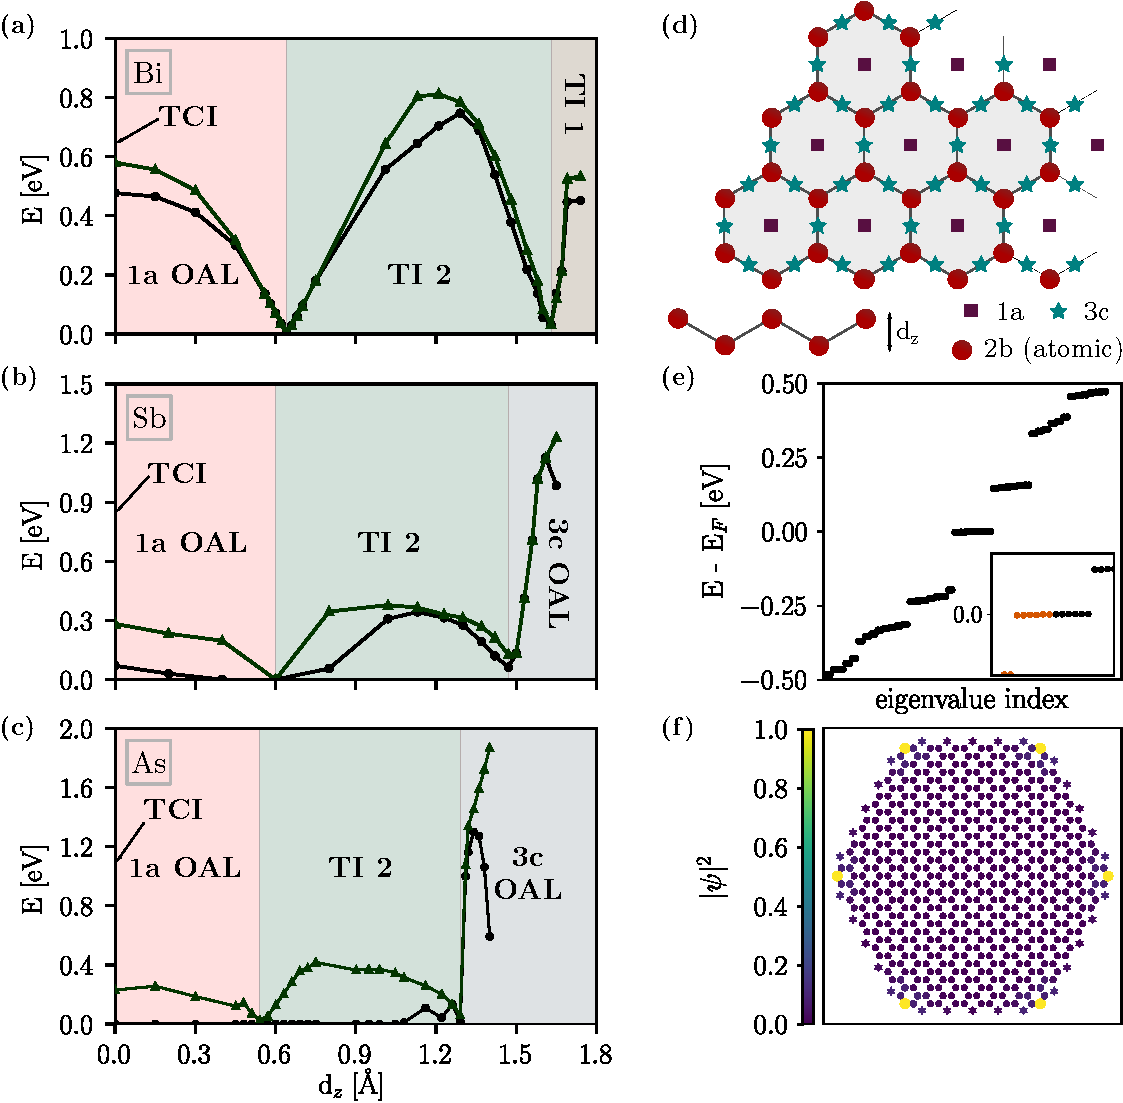
\includegraphics[width=\columnwidth]{oal_finite.pdf}
\caption[Energy gap as a function of the buckling parameter $d_z$, the Wyckoff positions of the space group 164, and results for a finite armchair-terminated flake of the $3c$ OAL]{Energy gap as a function of the buckling parameter $d_z$ for \textbf{(a)} bismuth, \textbf{(b)} antimony and \textbf{(c)} arsenic monolayers. The black line (circles) indicates the indirect gap, while the green line (triangles) indicates the direct gap. Top and side views of the lattice structure are illustrated in \textbf{(d)}, together with the Wyckoff positions of the space group 164. \textbf{(e)} Low-energy spectrum of a finite armchair-terminated flake of the $3c$ OAL. The inset presents the energies around the Fermi level, with filled states in orange. \textbf{(f)} The electronic densities of the corner states with color scale proportional to the normalized square modulus $|\psi_i|^2$ of the eigenstates (normalized with respect to the largest $|\psi_i|^2$). The tellurium atoms used for edge passivation are shown as stars.}
\label{fig:oal_finite}
\end{figure}

\begin{table}[H]
	\begin{tabularx}{\linewidth}{ | >{\centering\arraybackslash}  m{0.12\textwidth} || >{\centering\arraybackslash} m{0.05\textwidth}| >{\centering\arraybackslash} m{0.05\textwidth}| >{\centering\arraybackslash}  m{0.06\textwidth}| >{\centering\arraybackslash}  m{0.05\textwidth}| >{\centering\arraybackslash}  m{0.05\textwidth}| >{\centering\arraybackslash}  m{0.06\textwidth}|| >{\centering\arraybackslash}  m{0.25\textwidth} || >{\centering\arraybackslash} m{0.05\textwidth} |}
		\hline 
		phase & $\# \Gamma_2^{\mathcal{I}}$&  $\# M_2^{\mathcal{I}}$ & $[M^\mathcal{I}_2]$ & $\# \Gamma_2^{(3)}$ & $\# K_2^{(3)} $ & $[K^{(3)}_2]$  &  $\chi^{(3)}_{\mathcal{I}} = ([M^\mathcal{I}_2], [K^{(3)}_2])$ & $\Delta_{\textnormal{TI}}$ \\
\hline		
		TI 1 & 4 & 6 & 2 & 0 & 4 & 4  &  (2, 4)& 1 \\
\hline 
		TI 2 & 4 & 6 & 2 & 2 & 4 & 2 & (2,  2) & 1 \\
		\hline 
		$3c$ OAL & 2 & 6 & 4 & 2 & 4 & 2  & (4, 2) & 0 \\
		\hline 
		$1a$ OAL & 4 & 4 & 0 & 2 & 4 & 2 & (0, 2) & 0\\
		\hline 
	\end{tabularx} 
	\caption[Topological invariants and symmetry indicators $\chi^{(3)}_{\mathcal{I}}$ corresponding to different regions in the phase diagrams]{Topological invariants and symmetry indicators $\chi^{(3)}_{\mathcal{I}}$ corresponding to different regions in the phase diagrams: The symmetry indicators were calculated using the primitive 2-site unit cell of the honeycomb lattice (see Table~\ref{tab:band_reps} for a decomposition in terms of elementary band representations). The indices $\chi^{(3)}_{\mathcal{I}}$ allow for a more refined classification even of the strong TIs. We find that the $3c$ and $1a$ OALs differ in their inversion indicator $[M^\mathcal{I}_2]$ and thus, as explained in the main text, inversion-symmetric flakes built from their hexagonal unit cells differ by a protected corner charge equal to $1 \mod 2$.}
	\label{tab:sym_indicators}
\end{table}

We present the band representations of the space groups 164 (P$\bar{3}$m1) and 191 (P6/mmm) relevant for discussed materials. To deduce Wyckoff positions from which EBRs can be induced, we use data collected from the Bilbao Crystallographic Server~\cite{Aroyo2011183,Bilbao1, Bradlyn17, Vergniory17}. Note that we discard Wyckoff positions with non-zero $z$-component as they are irrelevant for a 2D geometry. The irreducible representations of bands at high-symmetry points were obtained using the \texttt{irrep} code~\cite{irrep-github, irrep-pap}, which relies on the double space group character tables~\cite{elcoro2017} published on the Bilbao Crystallographic server~\cite{bilbao-server}.
\begin{table}[!htbp]
\centering
\begin{tabularx}{\linewidth}{ | @{} >{\centering\arraybackslash} m{0.06\textwidth}  | >{\centering\arraybackslash} m{0.1\textwidth} |  >{\centering\arraybackslash} X | >{\centering\arraybackslash} X @{} | }
		\hline 
		 SG & phase & band representation & EBRs \\
		\hline
		164 & TI 1 & $(3\bar{\Gamma}_{8}\oplus 2\bar{\Gamma}_{9},2\bar{M}_{3}\bar{M}_{4}\oplus3\bar{M}_{5}\bar{M}_{6},2\bar{K}_{4}\bar{K}_{5}\oplus 3\bar{K}_{6})$ & --  \\
		\hline
		164 & TI 2 & $(2\bar{\Gamma}_{8}\oplus 2\bar{\Gamma}_{9}\oplus\bar{\Gamma}_{4}\bar{\Gamma}_{5},2\bar{M}_{3}\bar{M}_{4}\oplus3\bar{M}_{5}\bar{M}_{6},2\bar{K}_{4}\bar{K}_{5}\oplus 3\bar{K}_{6})$ & -- \\
		\hline
		164 & $3c$ OAL & $(3\bar{\Gamma}_{8}\oplus\bar{\Gamma}_{9}\oplus\bar{\Gamma}_{4}\bar{\Gamma}_{5},2\bar{M}_{3}\bar{M}_{4}\oplus3\bar{M}_{5}\bar{M}_{6},2\bar{K}_{4}\bar{K}_{5}\oplus 3\bar{K}_{6})$ &  $\bar{E}_{1}(2d)  \oplus\ {}^{1}\bar{E}_{g}^{2}\bar{E}_{g}(3c)  $  \\
		\hline
		164 & $1a$ OAL & $(2\bar{\Gamma}_{8} \oplus 2\bar{\Gamma}_{9} \oplus \bar{\Gamma}_{4} \bar{\Gamma}_{5}, 3 \bar{M}_3 \bar{M}_4 \oplus 2 \bar{M}_5 \bar{M_6}, 2 \bar{K}_4 \bar{K}_5 \oplus 3 \bar{K}_6)$ & $\bar{E}_{1g}(1a)  \oplus \bar{E}_{1u}(1a) \oplus \bar{E}_{1}(2d)  \oplus {}^{1}\bar{E}_{g}^{2}\bar{E}_{g}(1a) $ \\
		\hline \hline 
		191 & TCI  & $(\bar{\Gamma}_{7}\oplus \bar{\Gamma}_{8}\oplus\bar{\Gamma}_{9}\oplus\bar{\Gamma}_{11}\oplus \bar{\Gamma}_{12},3\bar{M}_{5}\oplus 2\bar{M}_{6},2\bar{K}_{7}\oplus \bar{K}_{8}\oplus 2\bar{K}_{9})$  & --  \\
		\hline
	\end{tabularx} 
	\caption[Band representations corresponding to distinct phases]{Band representations corresponding to distinct phases as shown in Fig.~\ref{fig:oal_finite}. '--' indicates that a given band representation cannot be written as a combination of EBRs.\label{tab:band_reps}}	
\end{table}

\subsection{Details on ab-initio calculations}
\label{sec:DFT}
Fully relativistic DFT calculations were performed via the Vienna \emph{ab initio} simulation package (VASP)~\cite{KresseFurth96-1, KresseFurth96-2} by employing the Perdew-Burke-Ernzerhof (PBE)~\cite{PBE-1, PBE-2} exchange-correlation functional and projected augmented-wave pseudopotentials~\cite{PAW-1, PAW-2}. For the self-consistent calculations, we used a $19 \times 19 \times 1$ $\mathbf{k}$ point grid generated for the Monkhorst-Pack method in case of Bi and Sb, and a $17 \times 17 \times 1$ mesh for As. The plane wave basis cutoff was set to 400 eV (Bi and Sb) or 350 eV (As). A finer grid of $30 \times 30 \times 1$ $\mathbf{k}$ points was used later on in order to obtain the energy gaps and band representations. The lattice parameters in the equilibrium configuration, which are in good agreement with previous reports~\cite{LattParamBi, LattParamSb, LattParamAs}, are summarized in Table~\ref{tab:latt_param}.

\begin{table}[!htbp]
\centering
\begin{tabular}{| c | c | c | c |}
\hline 
& Bi & Sb & As \\
\hline
$a$ [\AA] & 4.39 & 4.04 & 3.61 \\
\hline 
$d_{z}$ [\AA] & 1.74 & 1.65 & 1.40 \\ 
\hline
\end{tabular}
\caption[Lattice constant and buckling parameter for the unstrained (free-standing) buckled structures]{Lattice constant and buckling parameter for the unstrained (free-standing) buckled structures.}
\label{tab:latt_param}
\end{table}

For open flake calculations, we employed the Siesta code~\cite{Soler_2002}. We used pseudo-atomic orbitals (PAO) with a basis of double zeta plus polarization orbitals (DZP) and norm-conserving fully relativistic pseudopotentials from the PseudoDojo library~\cite{VANSETTEN201839}. The bulk crystal structure was terminated to obtain a hexagonal structure of 546 Sb atoms, and 30 Te atoms were added to the edges in order to passivate the edge states (as shown in Fig.~\ref{fig:oal_finite}~(f)). The distance between Te and edge Sb atoms was set to a value 3.02 \AA, which was determined from the structure relaxation of an armchair Sb ribbon with Te adatoms at the edge. The DFT data post-processing was performed with the \texttt{sisl} Python package~\cite{zerothi_sisl}. 

\begin{table}[H]
\begin{tabularx}{\linewidth}{| >{\centering\arraybackslash}  m{0.08\textwidth} | >{\centering\arraybackslash}  m{0.14\textwidth} | >{\centering\arraybackslash}  m{0.16\textwidth} | >{\centering\arraybackslash}  m{0.28\textwidth} | >{\centering\arraybackslash}  X |}
\hline
group & generators & classification & $Q_\mathrm{c} \mod 2$& same classification \\
\hline
1     &  -          & $\mathbb{Z}_1$ &$\{0\}$            & 4, 5, 8, 9, 10, 11, 12, 13, 27, 28, 29, 30, 31, 32, 33, 34, 35, 36               								\\ \hline
2     & $I$        & $\mathbb{Z}_2$ &$\{0,1\}$  & 7, 14, 15, 16, 17, 18, 39, 43, 44, 45, 46, 52, 62, 64                  									\\ \hline
3     & $C_2^z$    & $\mathbb{Z}_2$  &$\{0,1\}$ & 19, 20, 21, 24, 25                    													 \\ \hline
6     & $I, C_2^z$ & $\mathbb{Z}_2$ &$\{0,1\}$  & 40               																\\ \hline
22     & $C_2^x, C_2^y$ & $\mathbb{Z}_2$&$\{0,1\}$  &                  								   \\ \hline
23     & $\mathcal{M}_x, \mathcal{M}_y$ & $\mathbb{Z}_2$ &$\{0,1\}$ & 26                 								   \\ \hline
37     & $\mathcal{M}_x, \mathcal{M}_y, M_z$ & $\mathbb{Z}_2$ &$\{0,1\}$ & 47                					 			  \\ \hline
38     & $\mathcal{M}_x, I$ & $\mathbb{Z}_2$ &$\{0,1\}$ & 41, 42, 48                					 	  		\\ \hline
49    & $C_4^z$ & $\mathbb{Z}_4$ &$\{0,1/2,1,3/2\}$             & 52, 54, 56                   															\\ \hline
50    & $C_4^z I$ & $\mathbb{Z}_4$ &$\{0,1/2,1,3/2\}$             & 58, 60                   																 \\ \hline
51    & $C_4^z, I$ & $\mathbb{Z}_4$  &$\{0,1/2,1,3/2\}$            & 63                   																 \\ \hline
53    & $C_4^z, C_2^x, C_2^y$ & $\mathbb{Z}_4$  &$\{0,1/2,1,3/2\}$            & 62                   														 \\ \hline
55    & $C_4^z, \mathcal{M}_x, \mathcal{M}_y$ & $\mathbb{Z}_4$  &$\{0,1/2,1,3/2\}$            & 64                   														 \\ \hline
57    & $C_4^z I, C_2^x, C_2^y$ & $\mathbb{Z}_4$ &$\{0,1/2,1,3/2\}$             &                    														 \\ \hline
59    & $C_4^z I, \mathcal{M}_x, \mathcal{M}_y$ & $\mathbb{Z}_4$ &$\{0,1/2,1,3/2\}$             &                    															 \\ \hline
61    & $C_4^z, I, C_2^x, C_2^y$ & $\mathbb{Z}_4$ &$\{0,1/2,1,3/2\}$             &                    														 \\ \hline
65    & $C_3^z$ & $\mathbb{Z}_3$   &$\{0,2/3,4/3\}$          &                   																	 \\ \hline
67    & $C_3^z, C_2^x$ & $\mathbb{Z}_3$  &$\{0,2/3,4/3\}$            & 68                															 \\ \hline
69    & $C_3^z, \mathcal{M}_x$ & $\mathbb{Z}_3$  &$\{0,2/3,4/3\}$            & 70                																 \\ \hline
71    & $C_3^z, \mathcal{M}_x, I$ & $\mathbb{Z}_6$ &$\{0,1/3,2/3,1,4/3,5/3\}$            & 72                   															 \\ \hline
73    & $C_6^z$           & $\mathbb{Z}_6$  &$\{0,1/3,2/3,1,4/3,5/3\}$           &                    																 \\ \hline
74    &  $C_6^z I$          & $\mathbb{Z}_6$  &$\{0,1/3,2/3,1,4/3,5/3\}$            &                    															 \\ \hline
75    & $C_6^z, I$           & $\mathbb{Z}_6$  &$\{0,1/3,2/3,1,4/3,5/3\}$            &                    														 	\\ \hline
76    & $C_6^z, C_2^x$           & $\mathbb{Z}_6$   &$\{0,1/3,2/3,1,4/3,5/3\}$           &                    														 \\ \hline
77    & $C_6^z, \mathcal{M}_x$           & $\mathbb{Z}_6$   &$\{0,1/3,2/3,1,4/3,5/3\}$          &                    															 \\ \hline
78    & $C_6^z I, \mathcal{M}_x$           & $\mathbb{Z}_6$  &$\{0,1/3,2/3,1,4/3,5/3\}$            & 79                  														 \\ \hline
80    & $C_6^z, I, \mathcal{M}_x$           & $\mathbb{Z}_6$   &$\{0,1/3,2/3,1,4/3,5/3\}$           &                   														 \\ \hline
\end{tabularx}
\caption[Corner charge classification and topological indices of layer groups]{Corner charge classification and topological indices of $\mathrm{S}$. The boundary classification of any layer group $\mathrm{l}$ is given by that of the group $\mathrm{s} \in \mathrm{S}$, where $\mathrm{s}$ is the largest possible subgroup of $\mathrm{l}$ contained in $\mathrm{S}$. In the case where $\mathrm{l}$ contains non-symmorphic operations, its classification is the same as that of the layer group $\mathrm{l}'$ that consists of the symmorphic part of $\mathrm{l}$.}
\label{tab:relevantlayergroups}
\end{table}
